%----------
%	CONFIGURACIÓN DEL DOCUMENTO
%----------
\documentclass[12pt]{report} %fuente a 12pt

% Expresiones matemáticas
\usepackage{amsmath,amssymb,amsfonts,amsthm}

\usepackage{txfonts} 
\usepackage[T1]{fontenc}
\usepackage[utf8]{inputenc}

\usepackage[spanish]{babel}
\decimalpoint

\usepackage{float}
\usepackage{color}
\usepackage{multirow}
\usepackage{multicol}
\usepackage{graphicx}
\usepackage{fancyhdr}
\usepackage{url}
\usepackage[ruled,vlined,spanish]{algorithm2e}

\usepackage[hidelinks]{hyperref}


% DEFINICIÓN DE COLORES para portada y listados de código
\usepackage[table]{xcolor}
\definecolor{azulUC3M}{RGB}{0,0,102}
\definecolor{gray97}{gray}{.97}
\definecolor{gray75}{gray}{.75}
\definecolor{gray45}{gray}{.45}

% diseño de PIE DE PÁGINA
\usepackage{fancyhdr}
\pagestyle{fancy}
\fancyhf{}
\renewcommand{\headrulewidth}{0pt}
\rfoot{\thepage}
\fancypagestyle{plain}{\pagestyle{fancy}}

% MÁRGENES: 2,5 cm sup. e inf.; 3 cm izdo. y dcho.
\usepackage[
a4paper,
vmargin=2.5cm,
hmargin=3cm
]{geometry}

\theoremstyle{definition}
\newtheorem{definition}{Definición}[section]
\newtheorem{theorem}{Teorema}[section]
\renewcommand*{\proofname}{Demostración}
\renewcommand\qedsymbol{$\blacksquare$}
\newcommand{\norm}[1]{\left\lVert#1\right\rVert}
\newtheorem{prop}{Proposición}

\usepackage{mathtools}
\DeclarePairedDelimiter{\ceil}{\lceil}{\rceil}

% DISEÑO DE LOS TÍTULOS de las partes del trabajo (capítulos y epígrafes o subcapítulos)
\usepackage{titlesec}
\usepackage{titletoc}
\titleformat{\chapter}[block]
{\large\bfseries\filcenter}
{\thechapter.}
{5pt}
{\MakeUppercase}
{}
\titlespacing{\chapter}{0pt}{0pt}{*3}
\titlecontents{chapter}
[0pt]                                               
{}
{\contentsmargin{0pt}\thecontentslabel.\enspace\uppercase}
{\contentsmargin{0pt}\uppercase}                        
{\titlerule*[.7pc]{.}\contentspage}                 

\titleformat{\section}
{\bfseries}
{\thesection.}
{5pt}
{}
\titlecontents{section}
[5pt]                                               
{}
{\contentsmargin{0pt}\thecontentslabel.\enspace}
{\contentsmargin{0pt}}
{\titlerule*[.7pc]{.}\contentspage}

\titleformat{\subsection}
{\normalsize\bfseries}
{\thesubsection.}
{5pt}
{}
\titlecontents{subsection}
[10pt]                                               
{}
{\contentsmargin{0pt}                          
	\thecontentslabel.\enspace}
{\contentsmargin{0pt}}                        
{\titlerule*[.7pc]{.}\contentspage} 

%-------------
%	DOCUMENTO
%-------------

\begin{document}
\pagenumbering{roman}

%----------
%	PORTADA START
%----------	
\begin{titlepage}
	\begin{sffamily}
		\color{azulUC3M}
		\begin{center}
			\begin{figure}[H] %incluimos el logotipo de la Universidad
				\makebox[\textwidth][c]{
\includegraphics[width=16cm]{imagenes/Portada_Logo.png}}
			\end{figure}
			\vspace{1cm}
			\begin{Large}
				Máster Universitario en Ingeniería Matemática\\			
				2018-2019\\
				\vspace{1cm}		
				\textsl{Trabajo Fin de Máster}
				\bigskip
				
			\end{Large}
			{\Huge Procedimiento de vecinos más cercanos con matrices de distancias parcialmente observadas}\\
			\vspace*{0.5cm}
			\rule{10.5cm}{0.1mm}\\
			\vspace*{0.9cm}
			{\LARGE Aldo Ramón Franco Comas}\\ 
			\vspace*{1cm}
			\begin{Large}
				Tutor\\
				Andrés M. Alonso Fernández\\
				\vspace{2cm}
				Leganés, 2019\\
			\end{Large}
		\end{center}
		
		\vfill
		\color{black}
	
			\noindent
\includegraphics[width=4.2cm]{imagenes/creativecommons.png}\\
			Esta obra se encuentra sujeta a la licencia Creative Commons \textbf{Reconocimiento - No Comercial - Sin Obra Derivada}
			
	\end{sffamily}
\end{titlepage}

%----------
%	PORTADA END
%----------	

\vfill
\newpage %página en blanco o de cortesía
\thispagestyle{empty}	
\mbox{}

%----------
%	RESUMEN Y PALABRAS CLAVE START
%----------	
\chapter*{ABSTRACT}
\setcounter{page}{3}
The nearest neighbors procedure is a non-parametric procedure that is used for the classification of new observations using the distance matrix between the observations to be classified and the observations in the training sample. In this project, we obtain a k-NN procedure when for reasons of response time, computational cost (e.g., in extremely large datasets) or destructive test it is not possible to calculate the distances between the new observations and all the observations in the training sample. The cases in which the distance matrix in the training sample is completely or partially observed will be addressed. The proposed procedure is illustrated using two well known real datasets.\\ 

\textbf{Key Words:} Distance matrix, k-NN, ultrametric, additive and cluster.
\vfill
\newpage %página en blanco o de cortesía
\thispagestyle{empty}
\mbox{}

%----------
%	RESUMEN Y PALABRAS CLAVE END
%----------	

%----------
%	DEDICATORIA START
%----------	
\chapter*{Agradecimientos}
\setcounter{page}{5}
Quisiera agradecer a mis tíos por haberme apoyado en todo momento en esta aventura. A mis padres por darme ánimo a pesar de la distancia y aceptar cada decisión que he tomado. A mi primo que al final se ha convertido en un hermano menor y a las abuelas que he conocido por asumirme como si fuera otro nieto. También agradecer a AXA Seguros S.A. por permitirme usar ese magnífico clúster que tienen en su sede en Francia.\\
\begin{flushright}
	A todos, muchas gracias.
\end{flushright}
\vfill
\newpage %página en blanco o de cortesía
\thispagestyle{empty}
\mbox{}

%----------
%	DEDICATORIA END
%----------	

%----------
%	ÍNDICES
%----------	

%--
%Índice general
%-
\tableofcontents
\thispagestyle{fancy}

\newpage %página en blanco o de cortesía
\thispagestyle{empty}
\mbox{}

%--
%Índice de figuras. Si no se incluyen, comenta las líneas siguientes
%-
\listoffigures
\thispagestyle{fancy}

\newpage %página en blanco o de cortesía
\thispagestyle{empty}
\mbox{}

%--
%Índice de tablas. Si no se incluyen, comenta las líneas siguientes
%-
\listoftables
\thispagestyle{fancy}

\newpage %página en blanco o de cortesía
\thispagestyle{empty}
\mbox{}

%----------
%	TRABAJO
%----------	
\clearpage
\pagenumbering{arabic} % numeración con múmeros arábigos para el resto de la publicación	

\chapter{Introducción}

\section{Motivación del trabajo}
Desde tiempos remotos los conceptos de distancia y cercanía han estado presentes en nuestra vida diaria. Este es uno de los motivos por el cual el algoritmo k-NN (k-Nearest Neighbors o k-Vecinos más Cercanos) sea fácil de entender intuitivamente, incluso por personas que tengan poca base matemática. Es uno de los métodos no paramétricos de aprendizaje supervisado más simple. En lo que sigue, se presentan las características básicas del procedimiento k-NN.\\

Los datos de entrada tienen la forma $\left\lbrace (x_i,y_i) \right\rbrace$ donde $x_i$ es un vector de longitud $p$, donde están representados $p$ atributos para cada caso $i$, mientras que $y_i$ es la variable respuesta o etiqueta que toma el caso $i$, dicha variable puede ser un valor numérico como por ejemplo la edad, el salario, la estatura o el peso; también puede ser un valor categórico como el género, el tipo de contrato laboral o la tipología de riesgo de accidentes. Igualmente se necesita una distancia entre un caso $x_i$ y otro $x_j$ denotada por $d(x_i,x_j)$. Para cada nuevo caso $x_{0}$ se calculan las distancias $d(x_0,x_i)$ para todo $i=1,...,n$, siendo $n$ el total de casos en el conjunto de entrenamiento y se buscan los $k$ casos más cercanos.

\begin{itemize}
	\item En la clasificación k-NN, la salida generalmente es una clase. Al nuevo objeto se le asigna la clase más común entre sus $k$ vecinos más cercanos. Si $k = 1$, entonces el objeto simplemente se asigna a la clase de ese vecino más cercano.
	\item En la regresión k-NN, la salida usualmente es el promedio de los valores de los k vecinos más cercanos.
\end{itemize}

Existen otros procedimientos de asignación/clasificación y predicción como vecinos más cercanos ponderados donde se da mayor peso a estos últimos. Más detalles en \cite{weightedknn}.\\

\noindent Como ventajas principales del k-NN tenemos:
\begin{itemize}
	\item \underline{No paramétrico:} No hace suposiciones explícitas sobre la forma funcional de los datos, evitando los peligros de alejarse de la distribución subyacente de los mismos.
	\item \underline{Algoritmo simple:} Fácil de explicar y de comprender.
	\item \underline{Alta precisión:} Es bastante alta, sin embargo puede no ser competitiva en comparación con otros métodos de aprendizaje supervisado, como pueden ser la redes neuronales o las máquinas de vector soporte (SVM), que utilizan procesos de entrenamiento mucho más costosos computacionalmente.
	\item \underline{Evoluciona constantemente:} Dado que es un aprendizaje basado en casos el algoritmo se adapta inmediatamente a medida que recopilamos nuevos datos de entrenamiento. Esto permite que el algoritmo responda rápidamente a los cambios en la entrada durante el uso en tiempo real.
	\item  \underline{Fácil de implementar para problemas de múltiples clases:} La mayoría de los algoritmos son fáciles de implementar para problemas binarios sin embargo requieren un esfuerzo extra a la hora de ser implementados para múltiples clases, como puede ser el caso de las SVM, mientras que k-NN se ajusta a múltiples clases sin ningún esfuerzo adicional.
	\item \underline{Clasificación y regresión:} Una de las mayores ventajas del k-NN es que se puede usar tanto para problemas de clasificación como de regresión.
	\item \underline{Variedad de distancias:} Ofrece una alta flexibilidad a la hora de elegir cualquier distancia al construir el modelo.
\end{itemize}

\noindent Mientras que sus desventajas son:

\begin{itemize}
	\item \underline{Datos no balanceados:} No funciona bien en datos no balanceados. Si consideramos un problema de clasificación binario con las siguientes clases rojo y azul, y la mayoría de los datos de entrenamiento están etiquetados como rojo, entonces el modelo pronosticará casi siempre rojo. Esto podría resultar en la clasificación errónea de la clase menos representada.
	\item \underline{Sensibilidad a valores atípicos:} Es sensible a los valores atípicos, ya que simplemente elige a los vecinos según los criterios de distancia.
	\item \underline{Tratamiento con valores perdidos:} No tiene la capacidad de lidiar con el problema de valores perdidos en las variables independientes o regresoras.
	\item \underline{Computacionalmente costoso:} Puede ser muy fácil de implementar, pero a medida que crece el conjunto de datos, la velocidad del algoritmo disminuye rápidamente.
	\item \underline{Necesita características homogéneas:} Es recomendable que las características tengan la misma escala pues si una variable está dada en milésimas de unidades y el resto en unidades, esta variable tendrá un impacto muy grande a la hora de calcular las distancias.
	\item \underline{Maldición de la dimensión:} Bajo un amplio conjunto de condiciones, a medida que se aumenta la dimensionalidad, la distancia al punto de datos más cercano se acerca a la distancia al punto de datos más lejano, ver en \cite{knnMeaningful}.
\end{itemize}

Dado lo anterior se puede llegar a la conclusión de que en problemas donde $n$ es muy grande, como ocurre hoy día en la era del Big Data, calcular todas estas distancias para predecir no sea factible. Esta situación puede darse, por ejemplo, cuando, por razones de tiempo de respuesta, coste computacional (por ejemplo, en conjuntos de datos extremadamente grandes) o pruebas destructivas (análisis de ADN), no es posible calcular todas las distancias de las nuevas observaciones a todas las observaciones en la muestra de entrenamiento. En este trabajo, propondremos una solución para los casos en que no sea posible calcular todas las distancias del caso a clasificar a todos los elementos del conjunto de entrenamiento.

\section{Objetivos}
Proponer un procedimiento k-NN donde no sea necesario calcular todas las distancias cada vez que tengamos que predecir un punto nuevo. Dado que solamente podemos calcular un porcentaje de las distancias, las restantes deben ser imputadas, este es el problema al cual nos enfrentamos. Compararemos distintos enfoques que se han propuesto para completar matrices de distancias \cite{MetricNearnessProblemApplications} \cite{DeSoete1984}  \cite{Lapointe} en combinación con el procedimiento k-NN en términos del error del vector de distancias y del orden de vecinos resultantes. Los métodos también se compararan por el coste computacional aún sabiendo que esto último depende del ordenador, lenguaje y forma de implementación, aunque para esto siempre se tratará de programar de la manera más eficiente y clara. Todos los experimentos se realizaron usando \textbf{\textsf{R}} \cite{R} y todos los códigos desarrollados se pueden encontrar en el siguiente repositorio de  {\href{https://github.com/aldofranco91/TFM_Ing_Mat}{\underline{GitHub}} (\emph{https://github.com/aldofranco91/TFM\_Ing\_Mat}).

\section{Estructura del trabajo}
El resto del trabajo se estructura en los siguientes capítulos:

\begin{itemize}
	\item Capítulo 2: Se hace una revisión de la literatura sobre algoritmos que nos pueden servir para abordar nuestro problema. Además se plantean aquellas definiciones que nos serán de utilidad para la solución de nuestro problema. Se realizan pruebas mediante simulación para determinar cuál método arroja el mejor resultado.
	\item Capítulo 3: Se utiliza el método propuesto en el dataset MNIST \cite{mnist} para un problema de  clasificación de múltiples clases (10 clases) y en el dataset DIAMONDS para un problema de regresión.
	\item Capítulo 4: Se presentan las conclusiones y futuras líneas de trabajo.
\end{itemize}

\chapter{Metodología: Antecedentes y propuesta}

En este capítulo se presentan las definiciones y resultados que nos serán de utilidad para la búsqueda de un método que resuelva nuestro problema junto con una revisión bibliográfica de artículos que abordan problemas similares al nuestro como lo es el problema de la métrica más cercana o el problema de la inferencia filogenética. Se propone una solución basada en procedimientos clúster y se compara el desempeño de las distintas opciones mediante un estudio de simulación.

\section{Definiciones básicas}

\begin{definition}\label{distancias}
Para un conjunto de elementos $X$ una \textit{distancia} o \textit{métrica} es cualquier función o aplicación $d(a,b): X \times X \rightarrow \mathbb{R}$ que verifique las siguientes condiciones:	
	\begin{itemize}
		\item No negatividad: $\forall a,b \in X: d(a,b) \geq 0$.
		\item Coincidencia: $d(a,b)=0 \iff a=b$.
		\item Simetría: $\forall a,b \in X : d(a,b)=d(b,a)$.
		\item Desigualdad triangular: $\forall a,b,c \in X: d(a,b) \leq d(a,c) + d(c,b)$. \cite{Rudin}
	\end{itemize}
\end{definition}

\begin{definition}
	Sea $M = \left\lbrace m_{ij} \right\rbrace $ una matriz $n \times m$, se dice \textit{no negativa} cuando todas sus entradas son no negativas, es decir $m_{ij} \geq 0 \  \forall i,j $.
\end{definition}

\begin{definition}
		Sea $M$ una matriz $n \times n$, se dice que es \textit{matriz de disimilitud} si es una matriz no negativa, simétrica y con ceros en su diagonal principal.\cite{MetricNearnessProblemApplications}
\end{definition}

\begin{definition}
Sean $x$ e $y$ dos puntos de $\mathbb{R}^n$ se define la \textit{distancia Manhattan} \cite{distances} entre estos puntos como:
\begin{equation}
	d_1(x,y) = \sum_{i=1}^{n}\left| x_i-y_i \right|.
\end{equation}
\end{definition}

\begin{definition}
	Sean $x$ e $y$ dos puntos de $\mathbb{R}^n$ se define la \textit{distancia euclidiana o euclídea} \cite{distances} entre estos puntos como:
\begin{equation}
d_2(x,y) = \sqrt{\sum_{i=1}^{n}(x_i-y_i)^2}.
\end{equation}
\end{definition}

\begin{definition}
Sean $x$ e $y$ dos puntos de $\mathbb{R}^n$ se define la \textit{distancia de Chebyshev} \cite{distances} entre estos puntos como:
\begin{equation}
d_\infty(x,y) = \max_{i=1,...,n} (\left| x_i-y_i \right|) .
\end{equation} 
\end{definition}

\begin{definition}
Sean $x$ e $y$ dos puntos de $\mathbb{R}^n$ se define la \textit{distancia de Minkowski} \cite{distances} entre estos puntos como:
\begin{equation} 
d_p(x,y) = \left( \sum_{i=1}^{n}\left| x_i-y_i \right|^p\right)^{1/p}.
\end{equation} 
\end{definition}

Notemos que para $p=1$ tenemos la distancia Manhattan y para $p=2$ tenemos la distancia euclidiana. Mientras que si hacemos $p \rightarrow \infty$ obtenemos la distancia de Chebyshev.

\begin{definition}
	Sea $M = \left\lbrace m_{ij} \right\rbrace $ una matriz $n \times n$, se dice que es una \textit{matriz de distancias}, si es una matriz de disimilitud cuyas entradas satisfacen la desigualdad triangular. Esto es, $M$, es matriz de distancias si y solo si para toda terna de índices $(i,j,k)$ se verifica que \cite{MetricNearness}: 
 $$m_{ik} \leq m_{ij} + m_{jk}.$$
\end{definition}

\begin{definition}
Una matriz de distancias, $M = \left\lbrace m_{ij} \right\rbrace $, se dice \textit{aditiva}, cuando sus entradas verifican tanto la desigualdad triangular como la cuadrangular \cite{Buneman}:
$$m_{ij} + m_{kl} \leq \max[m_{ik}+m_{jl} ; m_{il}+m_{jk}] \quad \forall i,j,k,l. $$
\end{definition}

\begin{definition}
Una matriz de distancias $M$, se dice \textit{ultramétrica}, cuando es aditiva y sus entradas verifican la desigualdad ultramétrica \cite{Hartigan}:
$$ m_{ij} \leq \max[m_{ik};m_{jk}] \quad \forall \ i,j,k.  $$
\end{definition}

\begin{definition}
	Se llama \textit{cardinalidad} al número de elementos de un conjunto $A$ y se denota por $\left| A \right| $.\cite{cardinalidad}
\end{definition}

\begin{definition}
El \textit{índice o coeficiente de Jaccard} entre dos conjuntos $A$ y $B$ se define como la cardinalidad de la intersección de ambos conjuntos dividida por la cardinalidad de su unión.\cite{jacard}
\begin{equation}
J(A,B) = \dfrac{\left| A \cap B \right| }{\left| A \cup B \right|} = \dfrac{M_{11}}{M_{01} + M_{10} + M_{11}},
\end{equation}

\noindent donde

\begin{itemize}
	\item $M_ {00} + M_ {01} + M_ {10} + M_ {11} = n.$
	\item $M_ {11}$ representa el número total de casos donde A y B tienen un valor de 1.
	\item $M_{01}$ representa el número total de casos donde el valor de A es 0 y el valor de B es 1.
	\item $M_{10}$ representa el número total de casos donde el valor de A es 1 y el valor de B es 0.
	\item $M_ {00}$ representa el número total de casos donde A y B tienen un valor de 0.
\end{itemize}

\begin{table}[H]
	\centering
	\begin{tabular}{|c|c|c|c|}
		\hline
		\multicolumn{2}{|c|}{\multirow{2}{*}{}} & \multicolumn{2}{c|}{A} \\ \cline{3-4} 
		\multicolumn{2}{|c|}{}                  & 0          & 1         \\ \hline
		\multirow{2}{*}{B}          & 0         & $M_{00}$   & $M_{10}$  \\ \cline{2-4} 
		& 1         & $M_{01}$   & $M_{11}$  \\ \hline
	\end{tabular}
\end{table}

\end{definition}

El índice de Jaccard siempre toma valores entre $0$ y $1$, correspondiendo este último a la igualdad entre ambos conjuntos.\\

Es importante destacar que existe otra medida que se llama el \textit{coeficiente de coincidencia simple} (SMC) \cite{smc} o\textit{ coeficiente de similitud de Rand} que es muy similar al Jaccard pues se define como:

$$ SMC =  \dfrac{M_{00} + M_{11}}{M_{01} + M_{10} + M_{11}} .$$

\begin{definition}\label{mae}
Se define el \textit{error absoluto medio} (MAE), como:
$$ MAE=\dfrac{\sum\limits_{i=1}^{k}\left| \widehat{O}_{i} - O_{i}\right|}{k}, $$
donde $\widehat{O}_{i}$ son los valores estimados y $O_{i}$ los valores reales u observados, siendo $k$ la cantidad de valores a estimar.\cite{Error}
\end{definition}

\begin{definition}
	Sea $O$ la matriz original y $P$ la matriz pronosticada, se define la \textit{diferencia relativa entre estas matrices} como:
	$$ \dfrac{\norm{O-P}_2}{\norm{O}_2},$$
	donde $\norm{A}_2 = \sqrt{\sum\limits_{i=1}^{m}\sum\limits_{j=1}^{n}\left| a_{ij}\right|^2 }$.	
\end{definition}

\begin{definition}
	Sea $o$ el vector original y $p$ el vector pronosticado, se define la \textit{diferencia relativa entre estos vectores} como:
	$$ \dfrac{\norm{o-p}_2}{\norm{o}_2},$$
	donde $\norm{o}_2 = \sqrt{\sum\limits_{i=1}^{n}o_i^2}$.
\end{definition}

\section{El problema de la métrica más cercana}

Supongamos que tenemos una matriz $D$ de dimensión $n \times n$ cuyos elementos deberían cumplir las desigualdades triangulares pero, por errores de medición o incluso por omisión de algunas mediciones, estas desigualdades no se verifican. El \textit{problema de la métrica más cercana} consiste en encontrar una matriz $M$ cuyos elementos cumplan las correspondientes desigualdades triangulares y que $M$ esté próxima a la matriz $D$. Este problema ha sido estudiado en \cite{MetricNearnessProblemApplications} \cite{MetricNearness}  y puede formularse como sigue:

\begin{quotation}
Si hay $n$ puntos, podemos recoger las medidas en una matriz simétrica  \textit{D} de $n \times n$ cuya entrada $(j,k)$
representa la ``distancia'' entre los objetos $j$ y $k$. Luego, buscamos aproximar esta matriz por otra matriz \textit{M} cuyas entradas satisfacen las desigualdades triangulares. Es decir, $m_{ik} \leq m_{ij} + m_{jk}$ por cada tupla $(i,j,k)$. En otras  palabras se requiere una matriz de distancias  \textit{M} que sea la más cercana a una matriz de disimilitud dada  \textit{D} con respecto a alguna norma entre matrices. Específicamente, se busca una matriz de distancias \textit{M} tal que,

\begin{equation}
\textit{M} \in \left\lbrace argmin_{X \in M_N} \begin{Vmatrix} W \odot (X-D) \end{Vmatrix} \right\rbrace, \label{eq:1}
\end{equation}

\noindent donde $M_N$ es el conjunto de todas las matrices de distancias $n \times n$, este conjunto es cerrado y convexo. Por otra parte $W$ es una matriz $n \times n$ de pesos, simétrica y no negativa y $\odot$ denota la multiplicación elemento a elemento entre dos matrices. La matriz de pesos $W$ refleja nuestra confianza en las entradas de la matriz $D$. Por ejemplo, cuando cada $d_{ij}$ representa una medida con varianza $\sigma_{ij}^2$, podríamos establecer $w_{ij} = 1 / \sigma_{ij}^2 $ y si falta una entrada en $D$, se pone a cero el peso correspondiente. Generalmente se asume que todos los pesos son iguales a uno. En \cite{TheMetricNearnessProblem} se proponen algoritmos para resolver el problema (\ref{eq:1}) para las normas $L_1$, $L_2$ y $L_\infty$.

\end{quotation}

\begin{theorem} 
	La función $\norm{ W \odot (X-D)}$ siempre alcanza su mínimo en $M_N$. Además, cada mínimo local es un mínimo global. Si, además, la norma es estrictamente convexa y la matriz de pesos no tiene ceros o infinitos fuera de su diagonal, entonces hay un mínimo global único.
\end{theorem}

La demostración de este teorema se encuentra en \cite{MetricNearnessProblemApplications} haciendo uso de resultados expuestos en \cite{ConvexAnalysis}.\\

En principio, es posible utilizar cualquier norma entre matrices para este problema, pero lo analizaremos para las normas $l_p$. Con lo cual los problemas asociados son:

\begin{equation}
\min_{X \in M_N} \left[ \sum_{j \neq j}  \left| w_{jk}(x_{jk} - d_{jk}) \right| ^p  \right]^{1/p}  \quad  1 \leq p < \infty \label{p=1}
\end{equation}

\noindent y

\begin{equation}
\min_{X \in M_N} \max_{j\neq k} \left| w_{jk}(x_{jk} - d_{jk}) \right| \quad  p = \infty \label{p=inf}
\end{equation}

Para resolver los problemas \eqref{p=1} y \eqref{p=inf} puede parecer que se debería utilizar programación lineal (LP) cuando $p=1,\infty$, y programación convexa para $p\neq 1,\infty$, pero resulta que los requisitos de tiempo y almacenamiento de estos enfoques son prohibitivos.\cite{TheMetricNearnessProblem}\\

Siguiendo \cite{TheMetricNearnessProblem}, se planteará el algoritmo para $p=2$ puesto que este caso resulta ser el más simple y juega un papel fundamental en la resolución de los problemas para $p=1$ y $p=\infty$:

\begin{quotation}
Dado un vector de disimilitud $d$, deseamos encontrar su proyección ortogonal $m$ sobre el cono $M_n$. Definamos $e=m-d$ que representaría los cambios a las distancias originales y $b = -Ad$ que indica en qué medida se viola la desigualdad triangular. El problema (\ref{p=1}) se convierte en

\begin{equation} \label{problema}
\begin{aligned}
	\min &\: \norm{e}_2, \\
	\text{sujeto a:} &\: Ae \leq b.
\end{aligned}
\end{equation}

A partir del minimizador $e^*$, usamos la ecuación $m^* = d + e^*$ para recuperar el vector con la distancia óptima. Iniciamos el vector en $e=0$, y empezamos a recorrer todas las tuplas $(i,j,k)$. Supongamos que se incumple la desigualdad triangular, con lo cual $e_{ij}-e_{jk}-e_{ki} > b_{ijk}$. Deseamos remediar este incumplimiento haciendo un ajuste $l_2$ de $e_{ij}$, $e_{jk}$ y $e_{ki}$. En otras palabras, el vector $e$ se proyecta ortogonalmente sobre el conjunto de restricciones $\left\lbrace x : x_{ij} - x_{jk} - x_{ki} \leq b_{ijk} \right\rbrace $. Esto equivale a resolver:
\begin{equation}
\begin{aligned}
\min &\: \dfrac{1}{2}\left[ (x_{ij}-e_{ij})^2 + (x_{jk}-e_{jk})^2 + (x_{ki}-e_{ki})^2 \right],  \\
\text{sujeto a:} &\: x_{ij} - x_{jk} - x_{ki}=b.
\end{aligned}
\end{equation}

Sin embargo se verifica fácilmente que la solución del problema anterior está dada por:
\begin{equation} \label{sol}
\begin{aligned}
	x_{ij} &\leftarrow e_{ij} + \mu, \\
	x_{jk} &\leftarrow e_{jk} + \mu, \\
	x_{ki} &\leftarrow e_{ki} + \mu,
\end{aligned}
\end{equation}

\noindent con $\mu = \dfrac{-b + e_{ij} - e_{jk} - e_{ki}}{3}$. Por lo tanto, solo tres componentes del vector $e$ tienen que ser actualizados, y sus valores están dados por \eqref{sol}. \\

A su vez, fijamos la desigualdad de cada tupla donde no se cumpla la desigualdad triangular usando \eqref{sol}. También debemos introducir un término de corrección para guiar el algoritmo al mínimo global. Las correcciones tienen una interpretación simple en términos de la dualidad del problema de la minimización \eqref{problema}: cada variable dual corresponde al incumplimiento en una sola desigualdad triangular, y cada corrección individual resulta en una disminución de dicho incumplimiento. El procedimiento se repite hasta que ninguna tupla reciba una actualización significativa.

\end{quotation}

El Algoritmo \ref{algoritmo} muestra el esquema iterativo completo.\\

\begin{algorithm}[H] \label{algoritmo}
	\SetAlgoLined
	\SetKwInOut{Input}{Entrada}
	\SetKwInOut{Output}{Salida}
	\Input{$\textit{D}$: Matriz de disimilitud y $\epsilon$ la tolerancia.}
	\Output{$\textit{M} = argmin_{X \in M_N} \begin{Vmatrix} (X-D) \end{Vmatrix}_2$}
	
	\For{$1 \leq i < j < k \leq n$}
	{$z_{ijk} \leftarrow 0$}
		\For{$1 \leq i < j  \leq n$}
	{$e_{ij} \leftarrow 0$}
	$\delta \leftarrow 1 + \epsilon$
	
	\While{$\delta > \epsilon$}{
		\ForEach{Incumplimiento de la desigualdad triangular para $(i,j,k)$}
		{$b \leftarrow d_{ki}+d_{jk}+d_{ij}$ \\
			$\mu \leftarrow -\dfrac{1}{3}(b-e_{ij}-e_{jk}-e_{ki})$ \\
			$\theta \leftarrow \min\left\lbrace \mu,z_{ijk} \right\rbrace$ \\
	 		$e_{ij} \leftarrow e_{ij} + \theta$ \\
			$e_{jk} \leftarrow e_{jk} - \theta$ \\
			$e_{ki} \leftarrow e_{ki} - \theta$ \\
			$z_{ijk} \leftarrow z_{ijk} - \theta$
	}
$\theta \leftarrow \textit{Suma de todos los cambios en los valores de} \ e.$}
\Return $M=D+E$
	\caption{Algoritmo Triangle Fixing para $l_2$.}
\end{algorithm}
 \vspace{0.5cm}

En nuestras simulaciones utilizaremos $p=2$. El algoritmo para este valor está implementado en \textbf{\textsf{R}} en la librería $dtw$ (Dynamic Time Warping) \cite{dtw}. Según comunicación con el autor de dicho paquete estos algoritmos pueden fallar, sobre todo cuando $n$ es muy grande. En nuestro caso fallaba a partir de $n = 800$.\\

Llegados a este punto, nos preguntamos ¿qué relación tiene el problema de la métrica más cercana con nuestro problema? Si asumimos que conocemos todas las distancias entre todos los $n$ objetos en nuestra muestra de entrenamiento podemos crear una nueva matriz $(n+1) \times (n+1)$ donde la columna/fila $(n+1)$ serían las distancias del punto $x_0$ a las restantes teniendo en cuenta que tendremos un $l \%$ de distancias sin calcular y podemos utilizar el Algoritmo \ref{algoritmo} para imputar esos valores. A estos valores faltantes tenemos que darle algún valor inicial pues el algoritmo que se usa para resolver el problema de la métrica más cercana necesita valores numéricos.\\

\noindent Los primeros enfoques para imputar estos valores faltantes fueron:
\begin{itemize}
	\item $d(x_0,x_j) = 0$, siendo $j$ aquel objeto del cual no tenemos la distancia real. Este primer enfoque fue un total fracaso con lo cual no reportamos resultados pues en el tiempo de ejecución era extremadamente alto al igual que las diferencias relativa entre matrices y vectores.
	\item $d(x_0,x_j) = \dfrac{\sum\limits_{i=1}^{n}d(x_i,x_j)}{n}  \quad , i \neq j$.
	\item $d(x_0,x_j) = \text{mediana}(d(x_i,x_j)) \quad , \forall i \neq j$.
\end{itemize}

\noindent Para comparar las distintas propuestas de valores iniciales de las distancias desconocidas realizamos un estudio de simulación que consta de los siguientes pasos:
\begin{enumerate}
	\item Se generan $n = 800$ puntos de una distribución normal multivariante con $\mu = \vec{0}_p$ y $\sigma = I_p$, siendo $p=20$.
	\item Se calcula la matriz de distancias, usando la distancia euclidiana.
	\item Se genera un nuevo punto $x_0$ y se calculan las $n$ distancias.
	\item Se asumen conocidas las distancias de $x_0$ a $n(1-l) = 80$ puntos, $(l=0.9)$ y las restantes distancias se imputan usando los métodos descritos anteriormente, con lo cual tenemos una matriz de disimilitud $D$.
	\item Se aplica el triangle fixing a $D$ y nos devuelve una matriz $M$.
	\item Se calcula la diferencia relativa entre la matriz $M$ y la matriz de distancias original al igual que la diferencia relativa entre el vector de distancias correspondientes a $x_0$ en la matriz original y en $M$. También se registra el tiempo de cómputo.
	\item Todo lo anterior se hace $N = 2000$ veces.
\end{enumerate}

Se puede apreciar en la figura \ref{fig:MD1} las diferencias relativas entre las matrices que devuelve el algoritmo y las matrices originales, al igual que la diferencias relativas entre el vector que contiene las distancias originales y el que devuelve el algoritmo, ver figura \ref{fig:MD2}.

\begin{figure}[H]
	\centering
	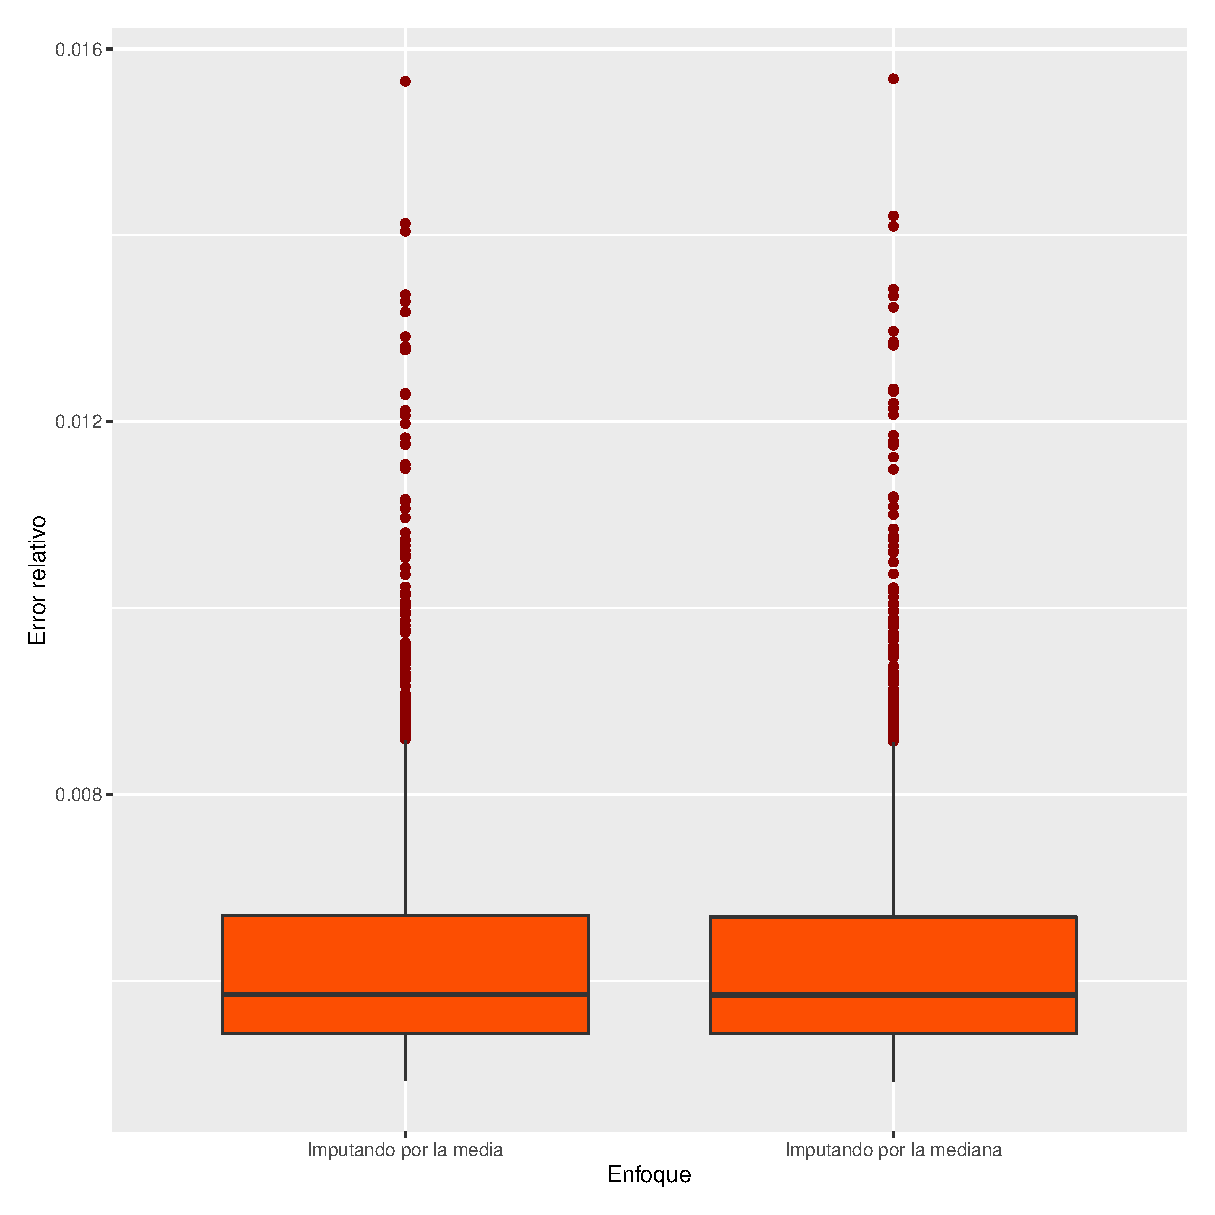
\includegraphics[scale=0.5]{imagenes/tf_imputation_mean_and_median_dif_relativa.eps}
	\caption{Diagramas de caja de las diferencias relativas entre la matriz de distancias original y la matriz imputada $M$.}
	\label{fig:MD1}
\end{figure}

\begin{figure}[H]
	\centering
	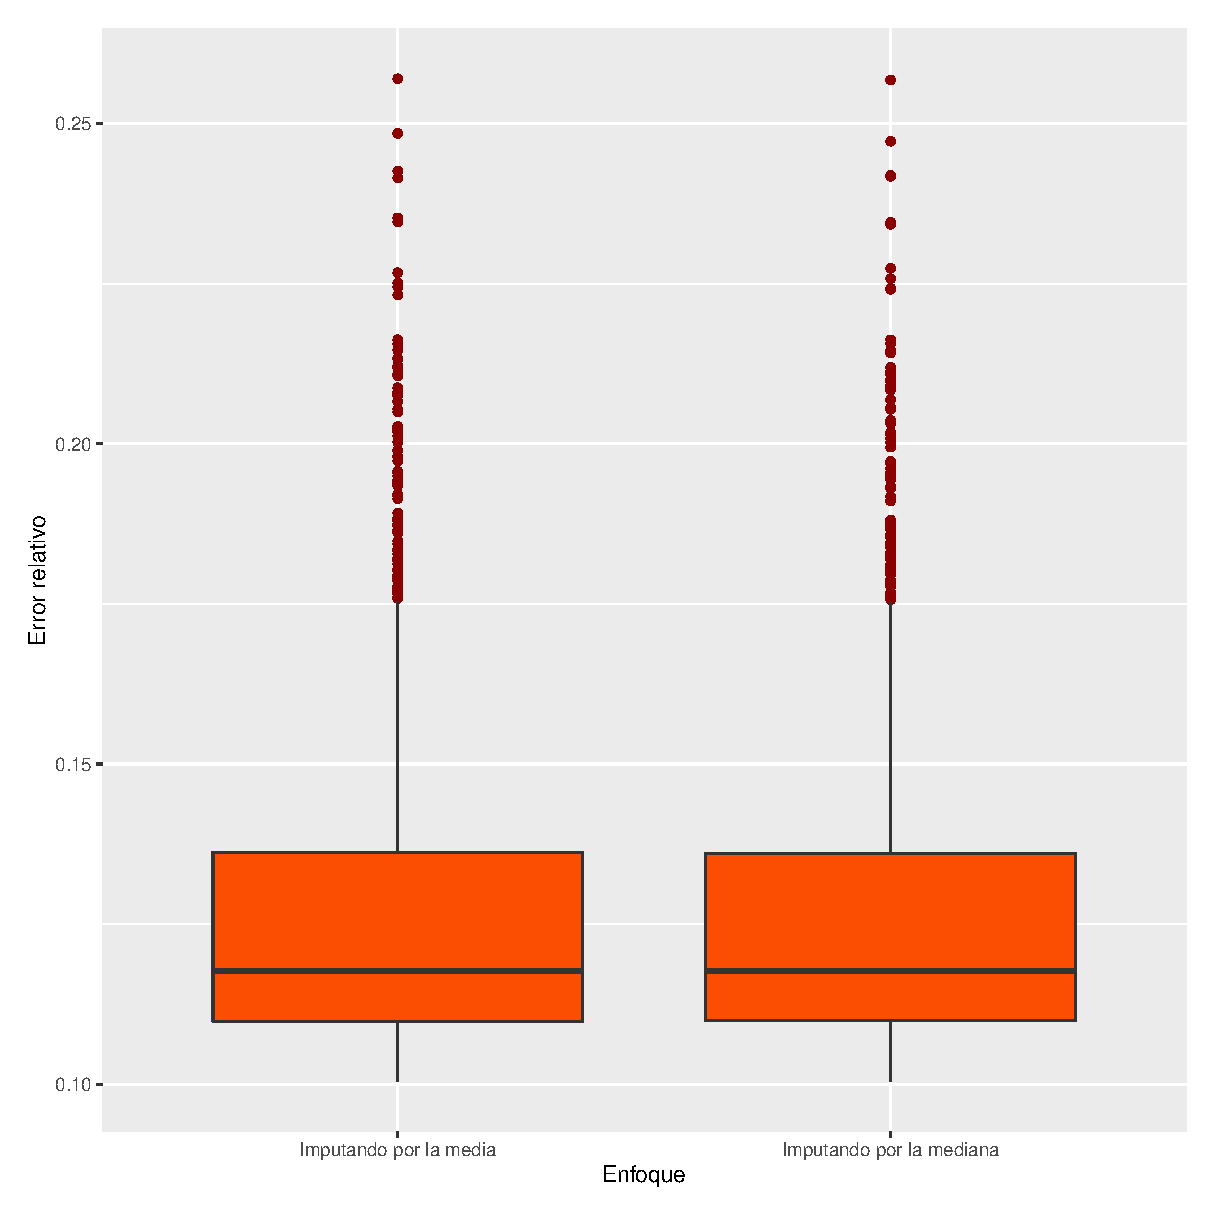
\includegraphics[scale=0.5]{imagenes/tf_imputation_mean_and_median_errores.eps}
	\caption{Diagramas de caja de las diferencias relativas entre las distancias reales e imputadas.}
	\label{fig:MD2}
\end{figure}

Estas grandes diferencias y altos costes en tiempo (como se puede apreciar en la figura \ref{fig:MD3}) viene dado por el hecho que nuestras imputaciones no verifican holgadamente las desigualdades triangulares, con lo cual el algoritmo tiene que iterar muchas veces. Por tanto debemos buscar una forma de mejorar estas aproximaciones iniciales.\\

\begin{figure}[H]
	\centering
	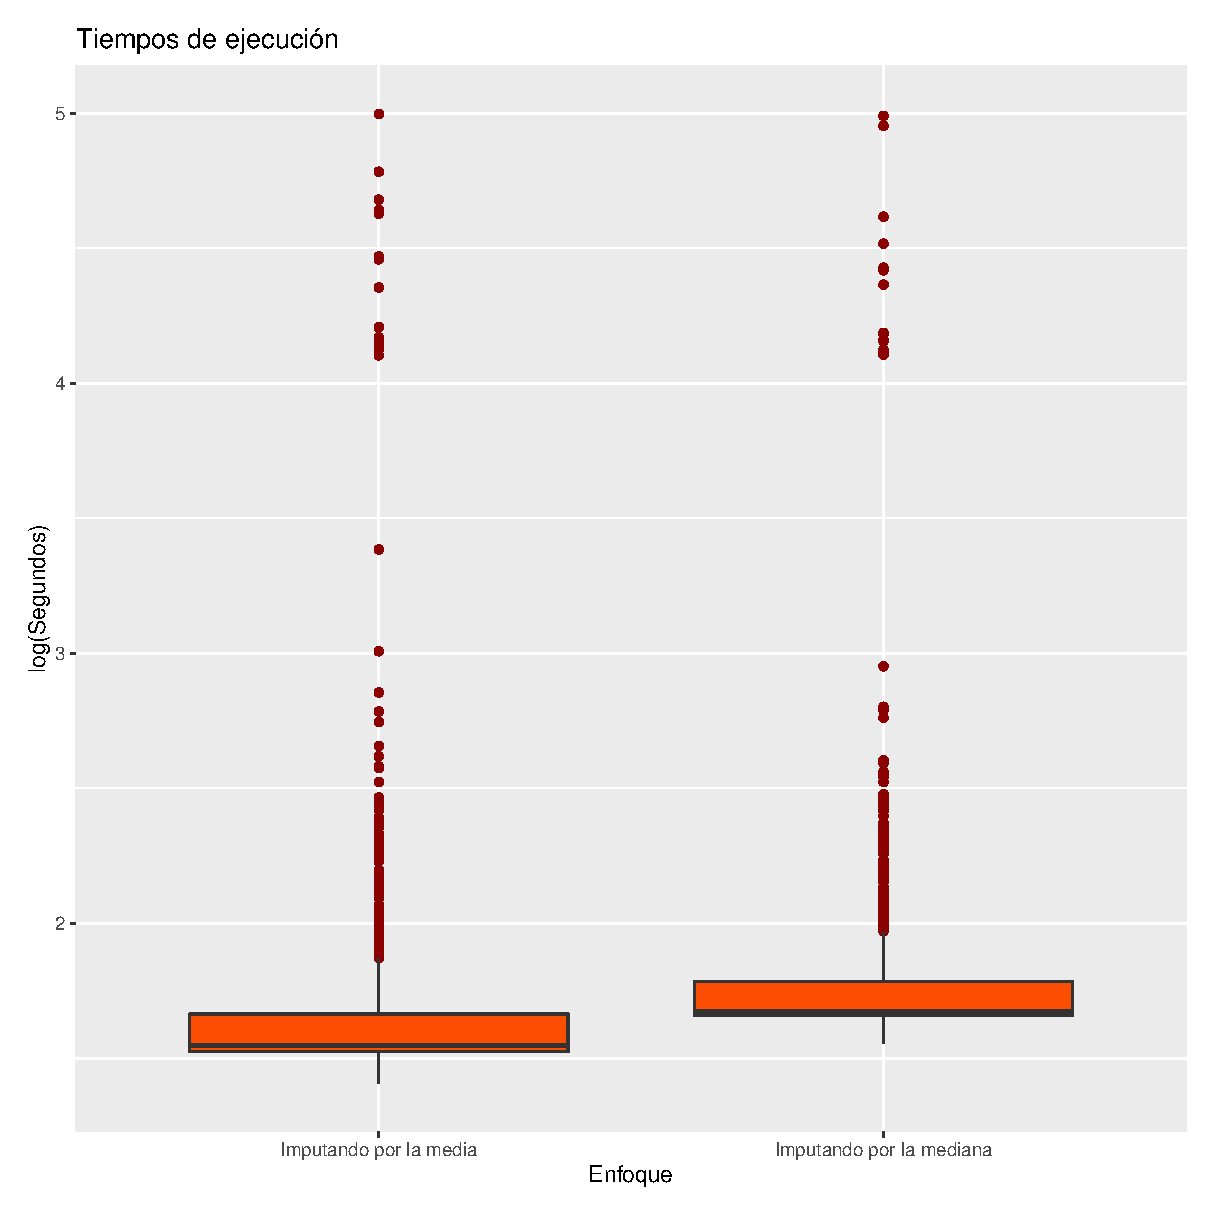
\includegraphics[scale=0.5]{imagenes/tf_imputation_mean_and_median_tiempo.eps}
	\caption{Diagramas de caja de los tiempos de ejecución para cada enfoque en escala logarítmica.}
	\label{fig:MD3}
\end{figure}

\subsection{Método propuesto}

De acuerdo a las restricciones impuestas a nuestro problema, sabemos que:

\begin{itemize}
	\item Las distancias $d(x_i,x_j)$ son conocidas $\forall i,j=\left\lbrace 1,...,n\right\rbrace$.
	\item Podemos calcular las distancias de $d(x_0,x_i)$ cuando $i \in I$ y $\left| I \right| << n$.
	\item No podemos calcular las $d(x_0,x_i)$ cuando $i \in I^c$.
	\item $\left| I \right| \approx (1-l)n$ y $\left| I^c \right| \approx ln$.  
\end{itemize}

Por otra parte haciendo uso de la desigualdad triangular tenemos:
\begin{equation}
d(x_0,x_{i^*}) \leq d(x_0,x_i) + d(x_i,x_{i^*}) \quad \forall i^* \in I^c,
\end{equation}
\indent por tanto obtenemos que:
\begin{equation}
d(x_0,x_{i^*}) \leq \min_{i \in I} \left\lbrace d(x_0,x_i) + d(x_i,x_{i^*}) \right\rbrace . 
\end{equation}

De igual forma, tenemos que:

\begin{equation}
d(x_i,x_{i^*}) \leq d(x_0,x_{i^*}) + d(x_0,x_{i})
\end{equation}
\noindent y
\begin{equation}
d(x_0,x_{i}) \leq d(x_0,x_{i^*}) + d(x_i,x_{i^*}),
\end{equation}
\noindent por tanto, obtenemos que:
\begin{equation}
\max_{i \in I} \left| d(x_0,x_{i}) - d(x_i,x_{i^*}) \right| \leq d(x_0,x_{i^*}).
\end{equation}
\noindent Finalmente,
\begin{equation}
\max_{i \in I} \left| d(x_0,x_{i}) - d(x_i,x_{i^*}) \right| \leq d(x_0,x_{i^*}) \leq  \min_{i \in I} \left\lbrace d(x_0,x_i) + d(x_i,x_{i^*}) \right\rbrace
\end{equation}
Como ya tenemos acotada $d(x_0,x_{i^*})$, asignaremos a dicha distancia la media de sus cotas:
\begin{equation}\label{eqn:somelabel}
d(x_0,x_{i^*}) = \dfrac{1}{2} \left( \min_{i \in I} \left\lbrace d(x_0,x_i) + d(x_i,x_{i^*}) \right\rbrace + \max_{i \in I} \left| d(x_0,x_{i}) - d(x_i,x_{i^*}) \right| \right).
\end{equation}

Cuando asignamos los valores imputados usando la expresión (\ref{eqn:somelabel}) para posteriormente aplicar el triangle fixing obtenemos que la matriz $D$ coincide con la matriz $M$ que devuelve dicho algoritmo. Con lo cual parece ser que esos valores imputados satisfacen todas las condiciones que debe verificar una matriz de distancia. Esto solo se ha comprobado mediante simulación utilizando $N=10000$ y valores de $l$ entre $0.6$ y $0.9$, pero no tenemos una prueba formal de esta conjetura.\\

Dado el coste computacional del algoritmo triangle fixing directamente imputaremos usando la expresión (\ref{eqn:somelabel}). Hasta ahora hemos seleccionados puntos al azar, en lo que sigue propondremos un método que nos ayude a mejorar estos resultados basándonos en métodos clúster.

\section{Clúster o agrupamiento}

El clustering o agrupamiento es una técnica de aprendizaje no supervisada que intenta encontrar relaciones entre variables pero no la relación que guardan con respecto a una variable objetivo, es decir sin hacer uso de las etiquetas. El conjunto de datos tiene que ser dividido automáticamente en clústeres, de manera que los objetos dentro del mismo clúster sean similares, mientras que los objetos de diferentes clústeres sean menos semejantes. No existe una definición general de clúster, lo que significa que diferentes enfoques pueden obtener diferentes clústeres del mismo conjunto de datos.\\

El motivo por el cual el agrupamiento será de gran importancia para nosotros está dado por el hecho de que hasta ahora hemos seleccionado los puntos a los cuales se le calculan las distancias de una forma totalmente aleatoria. Pero usaremos, la idea propuesta en \cite{EfficientkNN}, donde en un conjunto de datos muy grandes se decide aplicar k-NN por submuestras y cada submuestra es definida mediante un clúster. A continuación se puede ver un resumen de dicho algoritmo.\\

\begin{algorithm}[H] \label{algoritmo knn eficiente}
	\SetAlgoLined
	\SetKwInOut{Input}{Entrada}
	\SetKwInOut{Output}{Salida}
	\Input{Datos de entrenamiento y dato a clasificar $x_0$.}
	\Output{Etiqueta.}
	1. Producir $K$ clústeres, $C_1,C_2,...,C_K$. \\
	2. Calcular la distancia de $x_0$ a todos los centroides, $d(x_0,C_i) \; \forall i=1,...,K$. \\
	3. Buscar el centroide($C_i$) más cercano a $x_0$. \\
	4. Crear un nuevo conjunto de datos, correspondientes a los puntos que pertenecen a $C_i$.\\
	5. Usar estos datos como datos de entrenamiento para predecir $x_0$.
	\caption{Algoritmo k-NN para Big Data.}
\end{algorithm}
\vspace{0.5cm}

Existen muchos métodos para agrupar como la agrupación jerárquica, los métodos k-medias, PAM (Partitioning Around Medoids), y DBSCAN (Density-Based Spatial Clustering of Application with Noise). Estos son de los más conocidos y usados \cite{listacluster}, sin embargo dado el impacto del Big Data existen trabajos que intentan paralelizar estos procedimientos y escalar a conjuntos de datos más grandes.

\subsection{Agrupamiento jerárquico}

El agrupamiento jerárquico es una técnica de aprendizaje no supervisada, la cual busca construir una jerarquía de grupos. Las estrategias para agrupamiento jerárquico generalmente se dividen en dos tipos:

\begin{itemize}
	\item Aglomerativas: Este es un enfoque ascendente, cada observación comienza en su propio grupo, y los pares de grupos son mezclados mientras se sube en la jerarquía.
	\item Divisivas: Todas las observaciones comienzan en un grupo, y se realizan divisiones mientras se baja en la jerarquía. 
\end{itemize}

Los resultados del agrupamiento jerárquico son muchas veces presentados mediante un dendrograma que no es más que una representación gráfica en forma de árbol. En el caso general, la complejidad del agrupamiento aglomerativo es $O(n^3)$ lo cual es muy ineficiente cuando $n$ es grande, sin embargo el agrupamiento divisivo con búsqueda exhaustiva es $O(2^n)$ lo cual es mucho peor.\\

Para decidir qué grupos deberían ser combinados (tipo aglomerativo), o cuando un grupo debería ser dividido (tipo divisivo), es necesario una medida de disimilitud entre los conjuntos. Es importante recalcar que la elección de una métrica apropiada influirá en la forma de los grupos, ya que algunos conjuntos pueden estar cerca unos de otros de acuerdo a una distancia y más lejos de acuerdo a otra. En el cuadro \ref{tab:linkage}, presentamos las tres métricas más conocidas. \cite{clustermetodos}

\begin{table}[H] 
	\centering
	\caption{Criterios de agrupamiento jerárquico.} 
	\begin{tabular}{|c|c|}
		\hline
		Nombre                                           & Fórmula \\ \hline
		Agrupamiento de enlace máximo o completo.         & $ \max \left\lbrace d(x,y): x \in X, y \in Y \right\rbrace $ \\ \hline
		Agrupamiento de enlace mínimo o simple.            &     $ \min \left\lbrace d(x,y): x \in X, y \in Y \right\rbrace $     \\ \hline
		Agrupamiento de enlace promedio, o UPGMA. &   $\frac{1}{|X||Y|}\sum_{x\in X}\sum_{y\in Y}d(x,y)$      \\ \hline
	\end{tabular}
\label{tab:linkage}
\end{table}

A continuación se puede apreciar cómo diferentes tipos de enlaces nos devuelve diferentes resultados (se usó un punto de corte $K=5$), los conjuntos de datos fueron descargados de \cite{ClusteringDatasets} y se conocen como conjuntos de datos de juguete.

\begin{figure}[H]
	\centering
	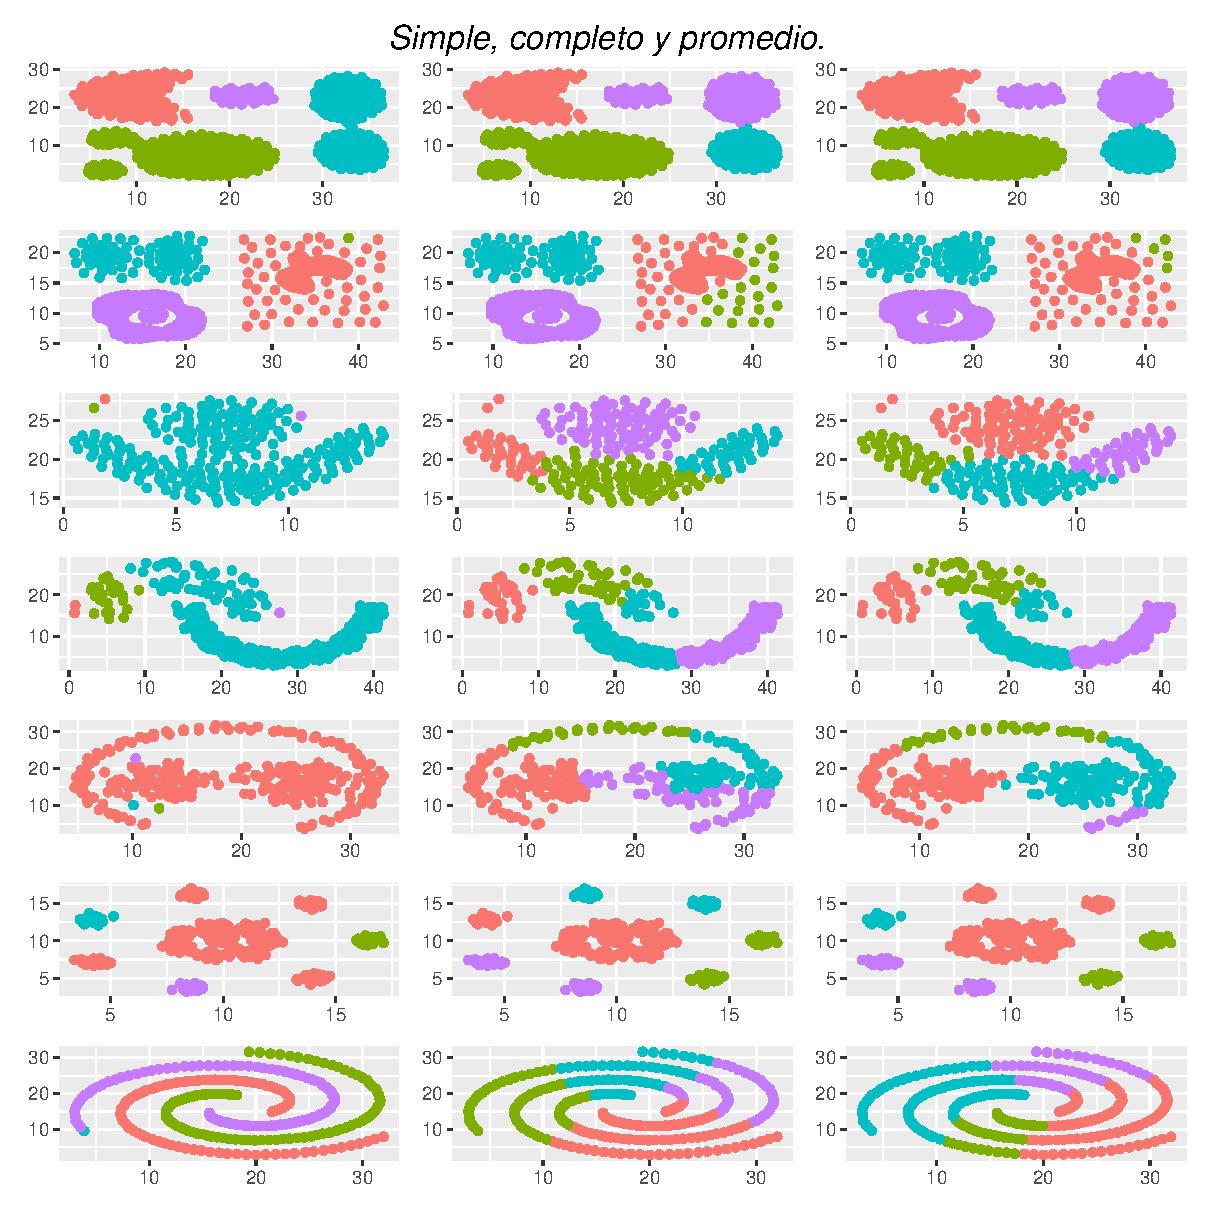
\includegraphics[scale=0.7]{imagenes/linkages.eps}
	\caption{Comparación de diferentes métodos de agrupamiento jerárquico.}
\end{figure}

\subsection{K-medias}

Otro de los algoritmos más usados es el K-medias, el cual tiene como objetivo crear $K$ grupos a partir de $n$ observaciones, en el que cada una pertenece a un grupo cuyo valor medio es el más cercano. Sean $(x_1,...,x_n)$ las observaciones, el algoritmo construye una partición de dichas observaciones, $C = \left\lbrace C_1,...,C_K \right\rbrace $, con el fin de minimizar la suma de los cuadrados dentro de cada grupo:
\begin{equation}
	\arg \min_C \sum_{i=1}^{K} \sum_{x_j \in C_i}  \begin{Vmatrix} x_j-\mu_i \end{Vmatrix}_2^2,
\end{equation}

\noindent donde $\mu_i$ es la media de $C_i$. Los $\left\lbrace \mu_i \right\rbrace $ se les llama centroides.\\ 

Desafortunadamente, aunque el agrupamiento de K-medias es bastante eficiente en tiempo computacional se sabe que es sensible a los valores atípicos. Por esta razón, a veces se utiliza la agrupación de K-medoids, donde se consideran objetos representativos dentro de cada clúster en lugar de los centroides.

\subsection{K-medoides}

K-medoides es una familia de algoritmos que escogen puntos del conjunto de datos como centros y trabaja con una métrica arbitraria de distancias. Es más robusto ante atípicos que K-medias porque minimiza una suma de disimilaridades (entre pares de puntos) en vez de una suma de distancias euclidianas cuadradas. Un medoide puede ser definido, como el objeto de un grupo cuya disimilaridad media a todos los objetos en el grupo es mínima.\\

La implementación práctica más común de K-medoides es el algoritmo Partición Alrededor de Medoides (PAM) y sea plantea como sigue:\\

\begin{algorithm}[H] 
	\SetAlgoLined
	\SetKwInOut{Input}{Entrada}
	\SetKwInOut{Output}{Salida}
	\Input{Seleccionar $K$ de los $n$ puntos como medoides.}
	\Output{$K$ medoides}
		Asociar cada punto al medoide más cercano.\\
		\While{Coste de la configuración disminuya}
		{
			\ForEach{medoide \textit{\underline{m}} y medoide \textit{\underline{o}}}
			{
				1. Intercambiar \textit{\underline{m}} y \textit{\underline{o}}, recalcular el coste (suma de la distancia de los puntos a sus medoids).\\
				2. Si el coste total de la configuración aumentó en el paso anterior, deshacer el intercambio.
			}
		}
	\caption{PAM (Partición Alrededor de Medoides)}
\end{algorithm}
\vspace{0.5cm}

Entre los algoritmos K-medoides que existen se encuentra el antes mencionado PAM que se considera uno de los más potentes, el CLARA y CLARANS. Sin embargo, PAM tiene el inconveniente de que funciona de manera ineficiente para conjuntos de datos grande (que es nuestro caso).\cite{pam_chungo}\\

Sin embargo existe una versión basado en K-medias para los medioides, este algoritmo se llama $fastkmed$ y está implementado en la librería \textit{kmed} \cite{kmed}. Además requiere la distancia entre cada par de objetos una sola vez y el resultado de varias simulaciones muestran que dicho método tiene mejor rendimiento que el agrupamiento K-medias. También se reduce significativamente el tiempo de ejecución con respecto al PAM con un rendimiento comparable, PAM es del orden de $O(k(n-k)^2))$ y el $fastkmed$ del orden de $O(nk)$ muy similar al K-medias. \cite{kmedarticle}\\

El algoritmo $fastkmed$ se define como sigue:\\

\begin{algorithm}[H] 
	\SetAlgoLined
	\SetKwInOut{Input}{Entrada}
	\SetKwInOut{Output}{Salida}
	\Input{Seleccionar $K$ de los $n$ puntos como medoides.}
	\Output{$K$ medoides.}
	1. Seleccione los medoides iniciales:
	\begin{itemize}
		\item Calcular la distancia entre cada par de objetos.
		\item Calcular $v_j$ para el objeto $j$ como sigue:
		$$ v_j =  \sum_{i=1}^{n}  \frac{d_{ij}}{\sum_{l=1}^{n} d_{il}}, \; j=1,...,n$$
		\item  Ordenar $v_j$ en orden ascendente. Seleccionar $k$ objetos teniendo los primeros $k$ valores más pequeños como medoides iniciales.
		\item Obtener el resultado del clúster inicial asignando cada objeto al medoide más cercano.
		\item  Calcular la suma de distancias de todos los objetos a sus medoides.
	\end{itemize}
	2. Actualizar medoides:
	\begin{itemize}
	\item Encontrar un nuevo medoide de cada grupo, que es el objeto que minimiza la distancia total a otro objeto en su clúster. Actualizar el medoide actual en cada grupo reemplazando con el nuevo medoide.
	\end{itemize}
    3. Asignar objetos a los medoides:
    \begin{itemize}
    	\item Asignar cada objeto al medoide más cercano y obtener el resultado del clúster.
    	\item Calcular la suma de la distancia de todos los objetos a sus medoides. Si la suma es igual a la anterior, detener el algoritmo y en caso contrario, volver al Paso 2.
    \end{itemize}
	\caption{Algoritmo fastkmed.}
\end{algorithm}
\vspace{0.5cm}

El algoritmo tiene una característica excelente, requiere que la distancia entre cada par de objetos se use una sola vez. Según los autores, el resultado de varias simulaciones que utilizan conjuntos de datos artificiales muestra que el $fastkmed$ tiene mejor rendimiento que el agrupamiento K-medias y reduce significativamente el tiempo de cálculo con respecto a PAM incluso con un rendimiento mejor. También la selección inicial de medoides empleado en dicho método funciona bastante bien en comparación con otros métodos.\cite{kmedarticle}

\begin{figure}[H]
	\centering
	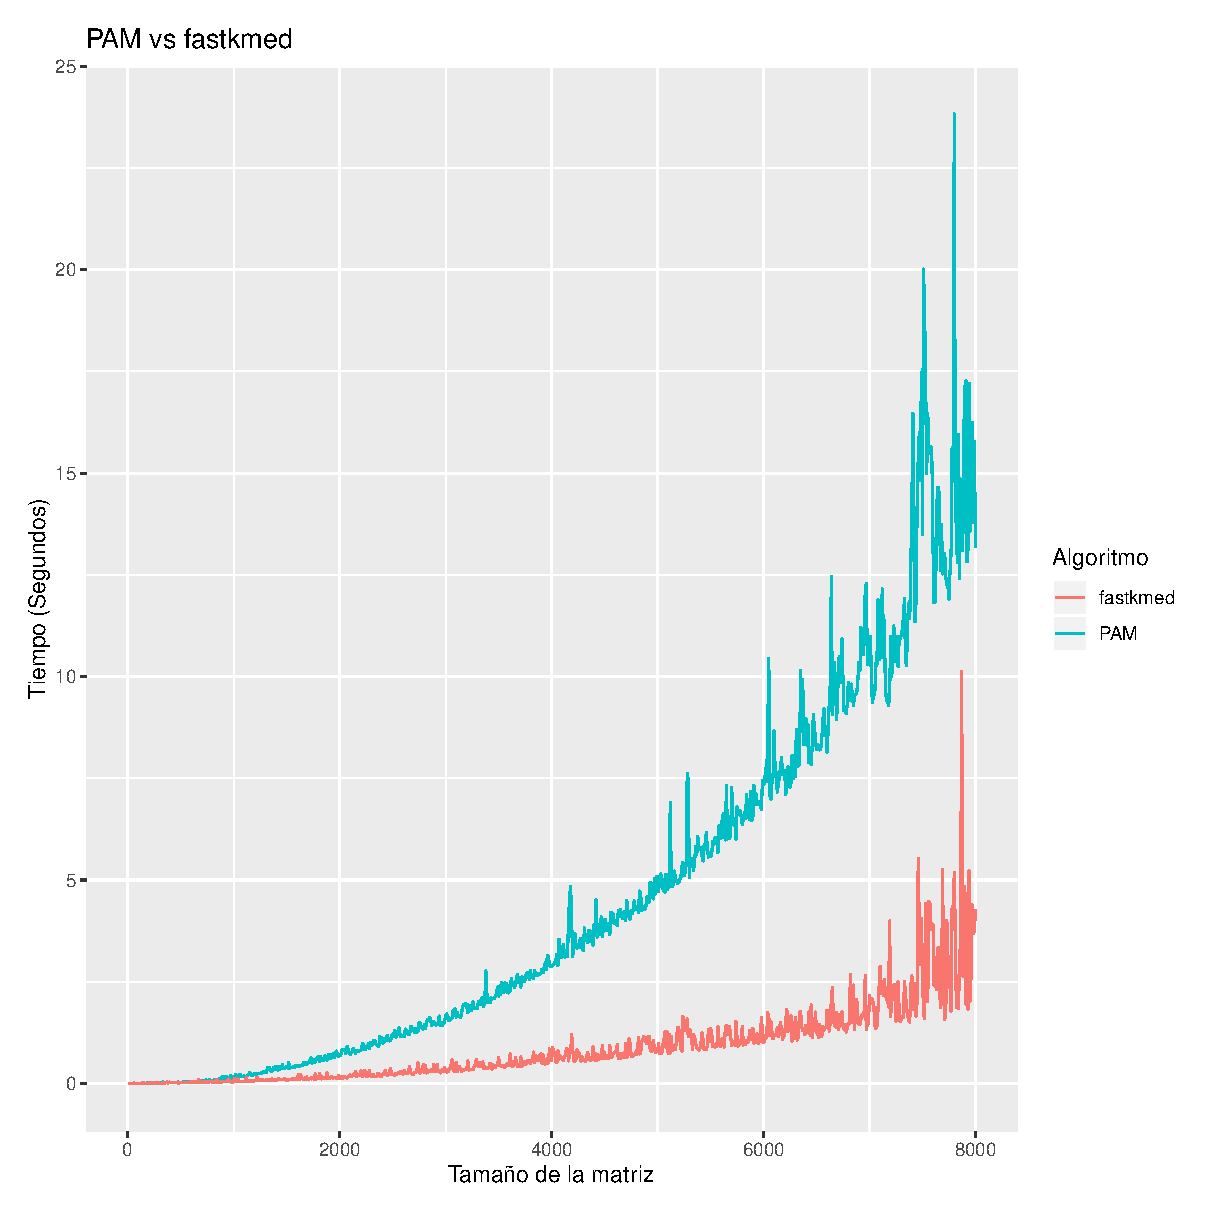
\includegraphics[scale=0.6]{imagenes/pam_vs_fastmed.eps}
	\caption{Comparación del PAM vs $fastkmed$ para $K=3$.}
	\label{fig:comparacion}
\end{figure}

En la figura \ref{fig:comparacion} mostramos el tiempo requerido por PAM y $fastkmed$. En la comparación el PAM se está compilando en su versión más rápida entre todas las propuestas \cite{pam} pues tiene diferentes versiones las cuales:
\begin{itemize}
	\item Reducen el tiempo de ejecución en un factor de $O(k)$.
	\item Permiten ejecutar múltiples intercambios por iteración, generalmente reduciendo el número de iteraciones.
	\item Permiten agregar optimizaciones menores y se espera que sea la variante más rápida.
\end{itemize}

Todas estas propuestas están implementadas para \textbf{\textsf{R}} haciendo uso de la librería $cluster$ \cite{cluster}.

\section{Aditivo y ultramétrico}

El problema de la inferencia filogenética a partir de conjuntos de datos que incluyen entradas incompletas o inciertas es uno de los temas más relevantes en biología sistemática.\cite{phylogenies} El objetivo es inferir filogenias a partir de datos evolutivos, incluida información faltante o incierta, por ejemplo, cuando las secuencias de nucleótidos o proteínas observadas contienen huecos o entradas faltantes.\\

Entre los diferentes algoritmos que existen sobre inferencia filogenética hay dos que se han usado para completar matrices de distancias $D$. Estos métodos han sido propuestos por \cite{DeSoete1984} y \cite{Lapointe} para ultramétricas, mientras que para matrices de distancias aditivas por \cite{Landry1996} y \cite{LandryLapointe}. Ambos algoritmos están implementados en \textbf{\textsf{R}}, en la librería $ape$ (Analyses of Phylogenetics and Evolution) \cite{ape}.\\

\begin{algorithm}[H] 
	\SetAlgoLined
	\SetKwInOut{Input}{Entrada}
	\SetKwInOut{Output}{Salida}
	\Input{Distancia parcial $d$ en el conjunto de $n$ taxones.}
	\Output{Distancia completa o parcial $d$ en el conjunto de $n$ taxones.}
	1. Contar el número de NAs en $d$, se define como $c$.\\
	2. \ForEach{$d(i,j)$ que sea NA de $d$}
	{
		$MinMax$ es la máxima entrada de $d$.\\
		\ForEach{$k$ tal que $d(i,k)$ y $d(j,k)$ son valores conocidos de $d$}
		{
			$Max = \max(d(i,k);d(j,k))$\\
			\If{$Max < MinMax$}{$Max = MinMax$}
		}
	\If{Si hay al menos un par conocido de entradas $d(i,k)$ y $d(j,k)$}
	{$d(i,j) = MinMax$\\
	$c = c-1$}
	}
	3. Si ha cambiado $c$, ir al punto 2.
	\caption{Algoritmo para distancias ultramétricas.}
\end{algorithm}
\vspace{0.5cm}

\begin{algorithm}[H] 
	\SetAlgoLined
	\SetKwInOut{Input}{Entrada}
	\SetKwInOut{Output}{Salida}
	\Input{Distancia parcial $d$ en el conjunto de $n$ taxones.}
	\Output{Distancia completa o parcial $d$ en el conjunto de $n$ taxones.}
	1. Contar el número de NAs en $d$, se define como $c$.\\
	2. \ForEach{$d(i,j)$ que sea NA de $d$}
	{
		$MinMax$ es la máxima entrada de $d$.\\
		\ForEach{$k,l$ tal que $d(i,k)$,$d(j,k),d(i,l)$,$d(j,l)$ y $d(k,l)$ son valores conocidos de $d$}
		{
			$Max = \max(d(i,k)+d(j,l);d(i,l) + d(j,k) - d(k,l))$\\
			\If{$Max < MinMax$}{$Max = MinMax$}
		}
		\If{Si al menos las entradas $d(i,k)$,$d(j,k),d(i,l)$,$d(j,l)$ y $d(k,l)$ son conocidas}
		{$d(i,j) = MinMax$\\
			$c = c-1$}
	}
	3. Si ha cambiado $c$, ir al punto 2.
	\caption{Algoritmo para distancias aditivas.}
\end{algorithm}
\vspace{0.5cm}

Estos algoritmos serán utilizados pues no requieren ningún tipo de imputación inicial. De hecho los valores faltantes deben definirse como NA para poder hacer uso de estos métodos. 

\section{Estudio de simulación}

En esta sección se compararán los diferentes métodos propuestos y para eso usaremos dos métricas, el MAE y el índice de Jaccard. Haremos simulaciones donde compararemos los resultados observación a observación, es decir en ningún momento analizaremos las etiquetas que pueden tener estas observaciones. Este ejercicio se hará en el próximo capítulo para los conjuntos de datos MNIST y DIAMONDS usando la mejor estrategia que salga de estas simulaciones.\\

El motivo por el cual usaremos ambas métricas viene dado por el hecho de que el índice de Jaccard presenta un inconveniente. Por ejemplo, supongamos que los vecinos más cercanos para una observación de validación $x_0$ son las observaciones $A=\left\lbrace 10,15,20,30\right\rbrace $ de la muestra de entrenamiento y obtenemos que un algoritmo nos devuelve los siguientes puntos más cercanos $B_1= \left\lbrace 10,15,20,35\right\rbrace $ y otro algoritmo los puntos $B_2= \left\lbrace 10,15,20,40\right\rbrace $ con lo cual se obtiene que 

\begin{equation}
J(A,B_1) = \dfrac{\left| A \cap B_1 \right| }{\left| A \cup B_1 \right|} = \dfrac{3}{5} = \dfrac{\left| A \cap B_2 \right| }{\left| A \cup B_2 \right|} = J(A,B_2).
\end{equation}

Vemos que el índice de Jaccard coincide y no permite diferenciar entre ambos resultados. Con el MAE seleccionaríamos el resultado con menor error de ``imputación'' de las distancias.\\

Primero estudiaremos el número de clústeres que debemos escoger de tal manera que el índice de Jaccard sea mayor. Es importante destacar que este problema es diferente al que resuelven métodos como el del codo (Elbow method), brecha (Gap) o el de la silueta (Silhoutte Method) sobre el número de clústeres presentes en un conjunto de datos.\\

\noindent Para encontrar un número ``óptimo'' de clústeres mediante simulación se hizo lo siguiente:
\begin{enumerate}
	\item Se generan $n = 3000$ puntos de una distribución normal multivariante con $\mu = \vec{0}_p$ y $\sigma = I_p$, siendo $p=50$.
	\item Se calcula la matriz de distancias, usando la distancia euclidiana.
	\item Se aplica $fastkmed$ a dicha matriz de distancias para diferentes valores de $K = (2,4,8,16,32,64,150,300) $, aquí el valor de $K$ es la cantidad de clústeres, de tal manera que se obtienen $K$ mediodes $\left\lbrace C_1,...,C_K\right\rbrace $.
	\item Se genera un nuevo punto $x_0$.
	\item  Calcular las distancias $d(x_0,C_i)$ con $i=1,...,K$ y se ordenan de menor a mayor.
	\item  En este punto ya hemos calculado $K$ distancias con lo cual las restantes se harán seleccionando de cada clúster más cercano hasta que se hayan calculado el número máximo de distancias $n(1-l) = 300$, pues $l = 0.9$.
	\item Para los diferentes valores de $K$ expuestos se calcula el índice de Jaccard y el MAE entre el conjunto real de puntos más cercano y el conjunto de puntos más cercano que se obtiene imputando, para $k=15$ vecinos.
	\item Se repiten los pasos $4-7$, $N=200$ veces.
\end{enumerate}

\begin{figure}[H]
	\centering
	\includegraphics[scale=0.7]{imagenes/{cluster_fastmed_knn_fijo_cluster_varia}.eps}
	\caption{Búsqueda de un valor ``óptimo'' de clústeres.}
	\label{fig:Kclsuter}
\end{figure}

Se puede observar en la figura \ref{fig:Kclsuter} que a medida que el número de clústeres aumenta el índice de Jaccard mejora, con lo cual a partir de este momento decidiremos usar como número de clústeres $K=150$ que es el valor correspondiente a $K = (n-ln)/2$, pues presenta menor variabilidad que $n-ln$ que sería el valor correspondiente a $K=300$. También observamos que el MAE decrece lentamente con el número de clústeres.\\

Se sabe que en k-NN elegir el valor del $k$, a veces, resulta ser una tarea nada fácil, con lo cual se decide usar desde $k=1$ hasta $k=\sqrt{n}$, usando solo los $k$ que tomen valores impares \cite{sqrtn}. Las siguientes comparaciones consideran estos valores de $k$ para evaluar el desempeño de las distintas propuestas en función de este parámetro esencial del procedimiento k-NN.\\ 

\noindent A continuación veremos si hay alguna mejora cuando imputamos usando puntos al azar o usando la idea del clúster, las simulaciones se hicieron de la siguiente forma:
\begin{enumerate}
	\item Se generan $n=5000$ puntos de una distribución normal multivariante con $\mu = \vec{0}_p$ y $\sigma = I_p$, siendo $p=50$.
	\item Se calcula la matriz de distancias, usando la distancia euclidiana.
	\item Se genera un nuevo punto $x_0$.
	\item Se calculan las distancias de $x_0$ a los $n$ puntos. 
	\item Se calculan las distancias de $x_0$ a $n(1-l)$ puntos al azar y también a la misma cantidad usando la idea del clúster antes mencionada con $K = (n-ln)/2$. En ambos casos las restantes distancias se imputan usando la expresión (\ref{eqn:somelabel}).
	\item Se ordenan dichas distancias y se extrae cuáles son los $k$ puntos más cercanos, el máximo valor que toma $k$ es $\sqrt{n}/2$ dado que $n$ es muy grande.
	\item Para diferentes valores de $k$ se calcula el índice de Jaccard y el MAE entre el conjunto de puntos más cercano real y el conjunto de puntos más cercano que se obtiene imputando usando ambos métodos.
	\item Todo lo anterior se hace $N=1000$ veces.
\end{enumerate}

\begin{figure}[H]
	\centering
	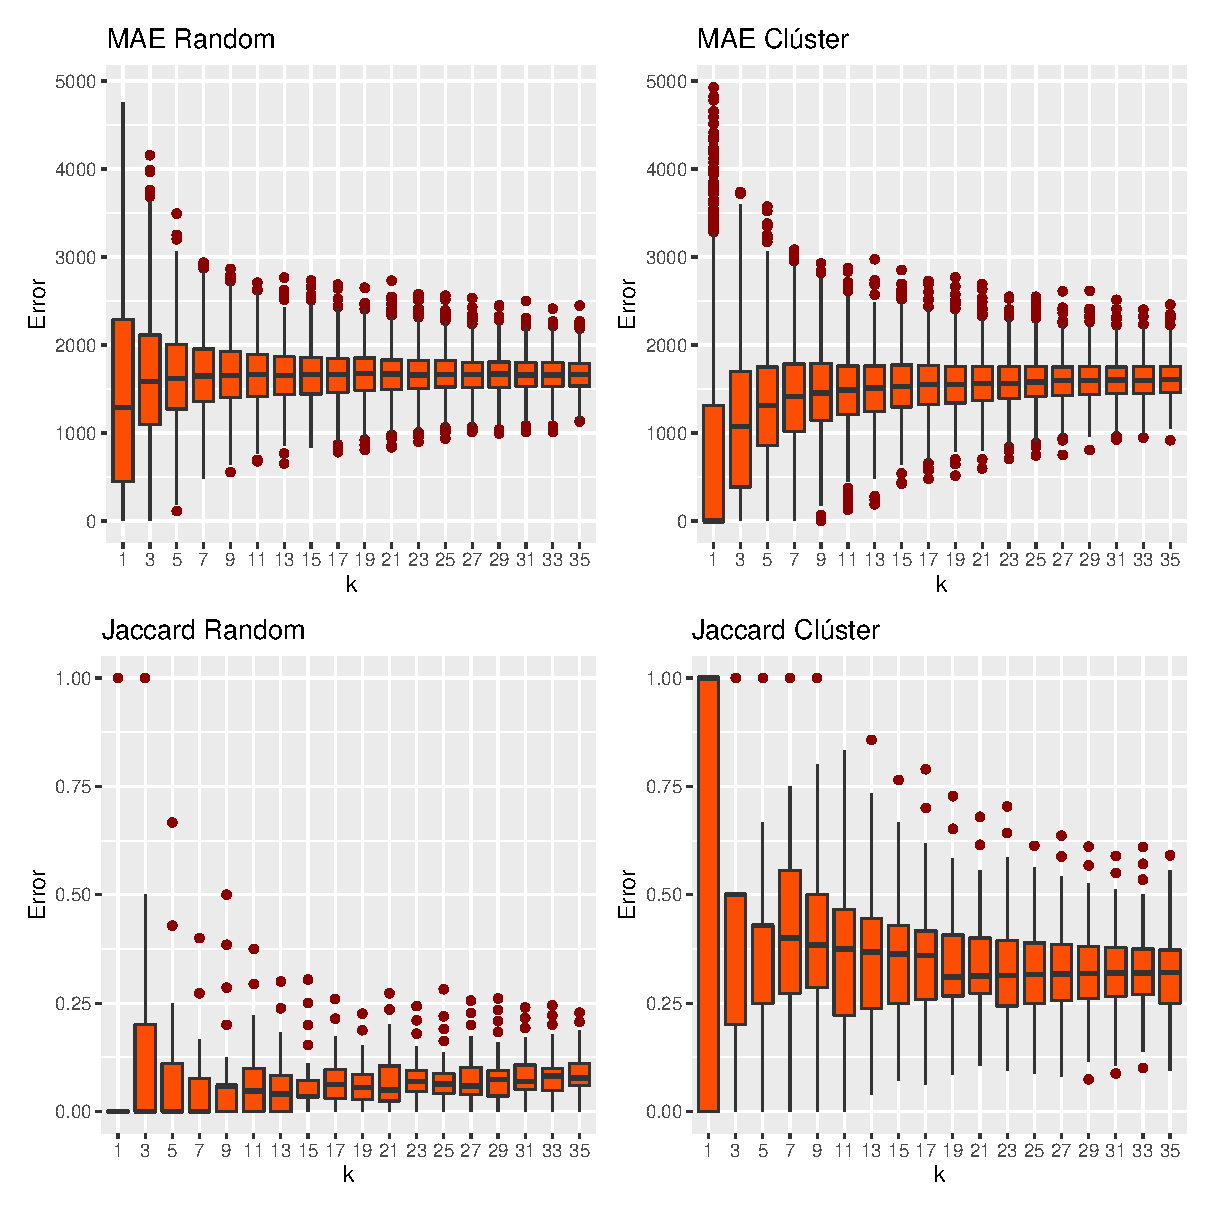
\includegraphics[scale=0.7]{imagenes/our_random_vs_our_cluster_fastmed.eps}
	\caption{Simulación comparando puntos al azar vs. puntos vía clúster.}
	\label{fig:clusterrandom}
\end{figure}

En la figura \ref{fig:clusterrandom} se puede apreciar claramente que calcular distancias al azar tiene un desempeño inferior al procedimiento basado en clústeres tanto para el MAE como para el índice de Jaccard. También hemos realizado la comparación entre los métodos ultramétrico y aditivo, viendo claramente que el ultramétrico es mejor, ver figura \ref{fig:ultrawin}.

\begin{figure}[H]
	\centering
	\includegraphics[scale=0.7]{imagenes/{Ultrametric_Additive}.eps}
	\caption{Comparación del procedimiento aditivo y ultramétrico para $n=1000$, $l=90\%$, $p=20$ y $N = 300$.}
	\label{fig:ultrawin}
\end{figure}

A continuación, se muestra una comparación entre el método ultramétrico y el método propuesto basado en clústeres, donde se puede apreciar que nuestro método tiene un mejor desempeño (ver figura \ref{fig:29}). 

\begin{figure}[H]
	\centering
	\includegraphics[scale=0.7]{imagenes/{our_and_ultrametric}.eps}
	\caption{Comparación ultramétrica vs. imputación vía clúster para $n=1000$, $l=90\%$, $p=20$ y $N = 300$.}
	\label{fig:29}
\end{figure}

Se observa que ambos enfoques de acuerdo al MAE no presentan una diferencia tan alta. Sin embargo, analizando el índice de Jaccard se puede ver que el método propuesto es superior al resto. Al método propuesto, en adelante, lo llamaremos como ``Imputación mediante clústeres''.

\chapter{Ejemplos con conjuntos de datos reales}

En este capítulo, ilustraremos el uso del procedimiento de imputación mediante clústeres en dos conjuntos de datos reales muy conocidos en la literatura del aprendizaje automático:
\begin{itemize}
	\item MNIST: Es una base de datos de dígitos escritos a mano. Son imágenes en blanco y negro.
	\item DIAMONDS: Es una base de datos que contiene los precios junto con otros diez atributos de varios tipos de diamantes.
\end{itemize}

\section{MNIST}
En esta sección, comprobaremos el procedimiento propuesto con el k-NN clásico usando un dataset real de clasificación. Usaremos la base de datos MNIST que consiste en imágenes en blanco y negro normalizadas cuyas dimensiones son de 28x28 píxeles en niveles de escala de grises de dígitos escritos a mano. El problema de clasificación, consiste en, dada una nueva imagen debemos predecir que número tiene escrito.\\

\begin{figure}[H]
	\centering
	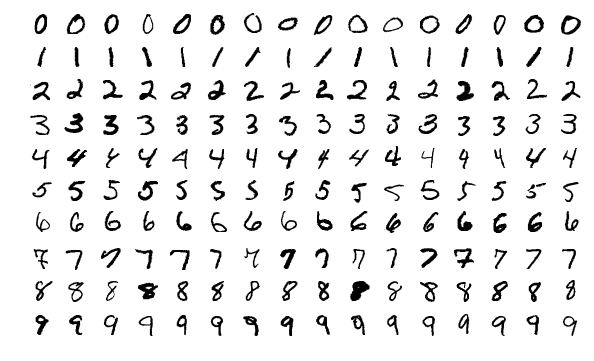
\includegraphics[scale=0.6]{imagenes/mnist.png}
	\caption{Imágenes seleccionadas del conjunto de datos de entrenamiento del MNIST.}
\end{figure}

Dicha base de datos fue descargada de {\href{https://www.kaggle.com/c/digit-recognizer/data}{\underline{Kaggle}} (\emph{https://www.kaggle.com/c/digit-recogn}\\  
\emph{izer/data}), consta de $42000$ observaciones, de las cuales dejaremos el 75$\%$ para entrenar y validar y las restantes para probar nuestro método. Esta división se hizo usando un reparto estratificado entre las muestras de entrenamiento y de prueba \cite{caret}.\\

Las razones para utilizar un muestreo estratificado en lugar de un muestreo aleatorio simple viene dado por \cite{hyndmandatapartition}:

\begin{itemize}
\item Mantener una distribución similar de las etiquetas originales en el nuevo subconjunto.
\item Para muchas aplicaciones, las mediciones se vuelven más manejables cuando la población se agrupa en estratos.
\item A menudo es deseable tener estimaciones de los parámetros de la población para todos los subgrupos.
\end{itemize}

\begin{figure}[H]
	\centering
	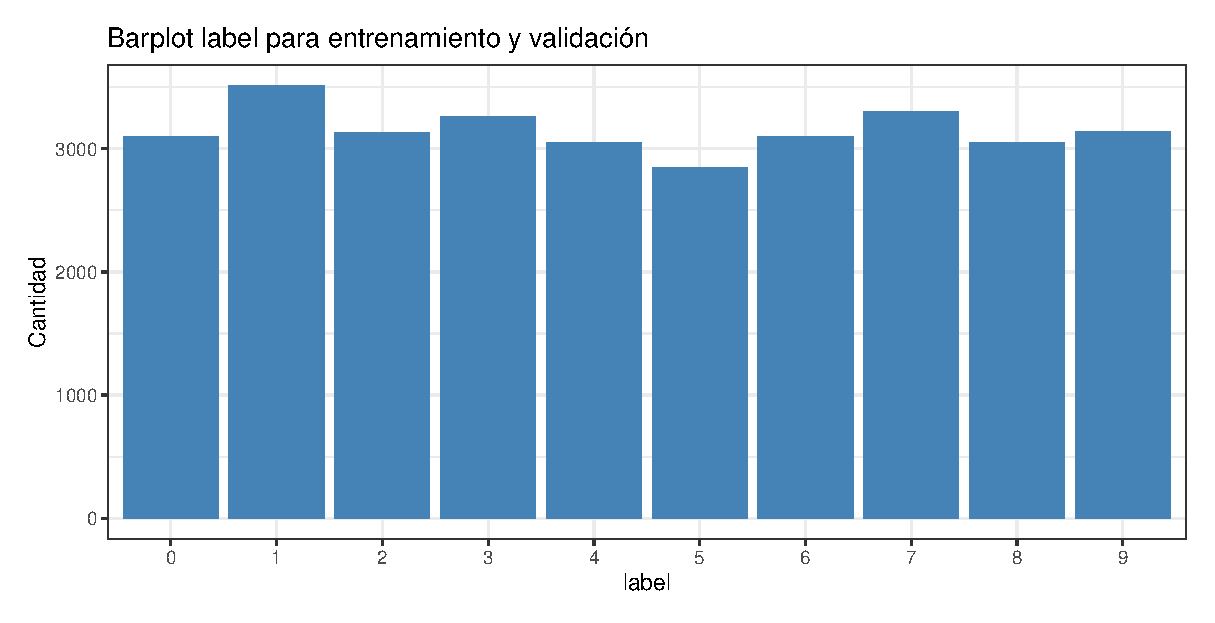
\includegraphics[scale=0.6]{imagenes/mnisttrain.eps}
	\caption{Frecuencia de las etiquetas de datos de entrenamiento y validación del MNIST.}
	\label{fig:label1}
\end{figure}

\begin{figure}[H]
	\centering
	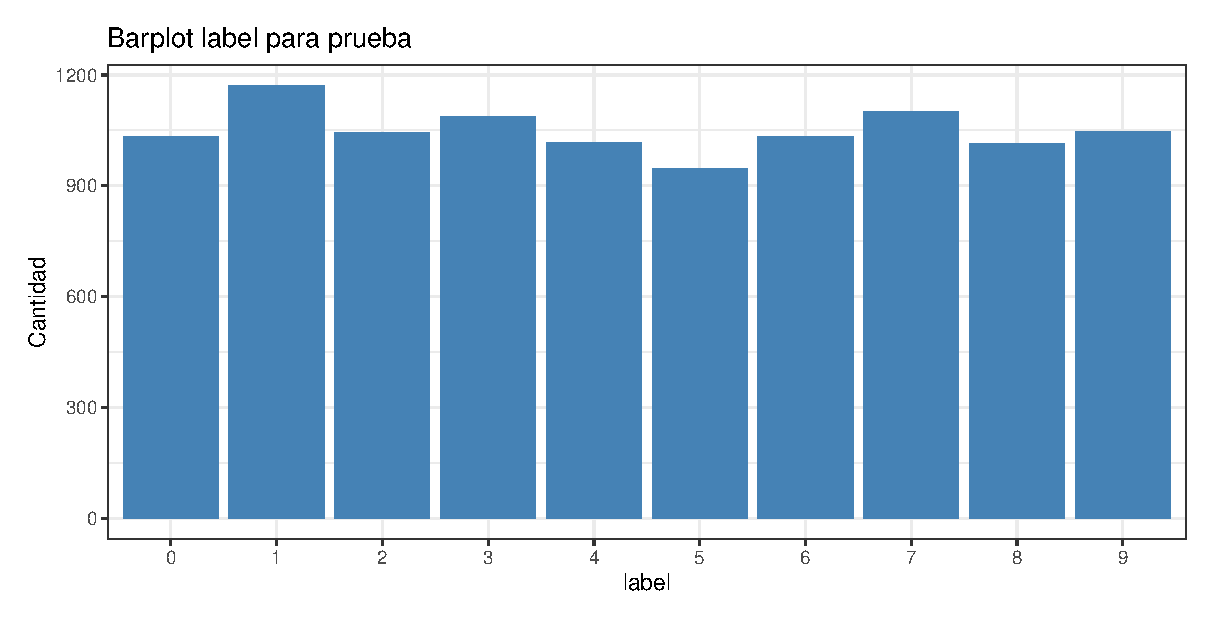
\includegraphics[scale=0.6]{imagenes/mnisttest.eps}
	\caption{Frecuencia de las etiquetas de datos de prueba del MNIST.}
	\label{fig:label2}
\end{figure}

Como se puede apreciar en las figuras \ref{fig:label1} y \ref{fig:label2} el conjunto de datos está balanceado con lo cual evitamos este problema, que es un punto débil que presenta k-NN como se había mencionado anteriormente. En caso de que fuera un dataset no balanceado se recomienda hacer data augmentation. Esta técnica es muy común a la hora de clasificar imágenes y no es más que tomar una imagen y crear nuevas muestras rotando, dilatando, trasladando o agregando ruido blanco a la original, ver figura \ref{fig:dataaug}.

\begin{figure}[H]
	\centering
	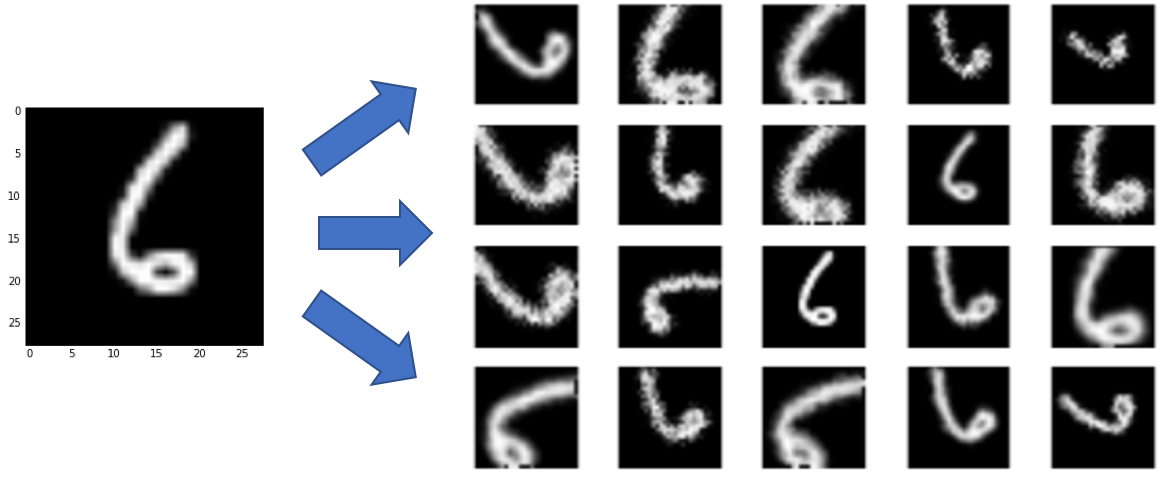
\includegraphics[scale=0.6]{imagenes/dataaug.png}
	\caption{Ejemplo de data augmentation para una muestra seleccionada del MNIST.}
	\label{fig:dataaug}
\end{figure}

Para la búsqueda del valor óptimo de $k$, se utilizó el procedimiento de validación cruzada con $5$ submuestras del conjunto de entrenamiento y validación donde se obtiene una precisión del $96.14\%$ siendo el mejor valor $k=3$, ver figura \ref{fig:modelo1}.

\begin{figure}[H]
	\centering
	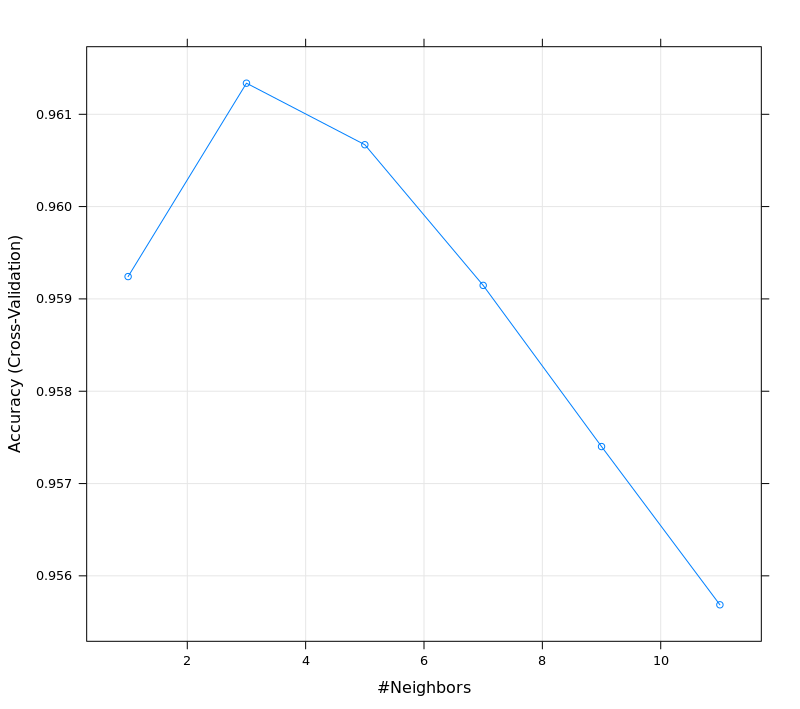
\includegraphics[scale=0.6]{imagenes/knn.png}
	\caption{Selección del parámetro $k$ del k-NN en datos de entrenamiento y validación del MNIST.}
	\label{fig:modelo1}
\end{figure}

Usando ahora este valor de $k$ predecimos las etiquetas para los valores de la muestra de prueba usando el k-NN donde se obtiene una precisión del $96.98\%$ con la siguiente matriz de confusión:

\begin{table}[H]
	\centering
	\caption{Matriz de confusión del MNIST usando k-NN($k=3$).}
	\label{tab:confussion matrix mnsit}
	\begin{tabular}{|c|c|c|c|c|c|c|c|c|c|c|}
		\hline
		& \multicolumn{10}{c|}{Referencia}                                 \\ \hline
		Predicción & 0    & 1    & 2    & 3    & 4   & 5   & 6    & 7    & 8   & 9    \\ \hline
		0          & 1024 & 0    & 4    & 2    & 1   & 4   & 6    & 2    & 1   & 6    \\ \hline
		1          & 0    & 1161 & 8    & 1    & 7   & 1   & 0    & 6    & 10  & 2    \\ \hline
		2          & 2    & 4    & 1002 & 4    & 0   & 2   & 2    & 3    & 4   & 2    \\ \hline
		3          & 1    & 0    & 5    & 1043 & 0   & 8   & 1    & 0    & 18  & 10   \\ \hline
		4          & 0    & 1    & 0    & 0    & 985 & 0   & 0    & 1    & 3   & 8    \\ \hline
		5          & 0    & 1    & 1    & 20   & 0   & 920 & 6    & 0    & 16  & 6    \\ \hline
		6          & 5    & 0    & 0    & 1    & 8   & 11  & 1019 & 0    & 5   & 0    \\ \hline
		7          & 0    & 3    & 21   & 5    & 3   & 0   & 0    & 1083 & 5   & 10   \\ \hline
		8          & 0    & 1    & 1    & 6    & 1   & 0   & 0    & 0    & 941 & 1    \\ \hline
		9          & 1    & 0    & 2    & 5    & 13  & 2   & 0    & 5    & 12  & 1002 \\ \hline
	\end{tabular}
\end{table}

Observando la matriz anterior podemos notar que los casos donde más falla el procedimiento son en etiquetas similares, por ejemplo el $7$ con el $2$ y el $5$ con el $8$.\\

Para este ejercicio, trabajamos con $l = 0.75$, lo que significa que solo podemos calcular el $25\%$ de las distancias. Las restantes fueron imputadas usando el método propuesto, donde el número de clústeres es $K = \dfrac{n-ln}{2} = 3938$. De esta forma se obtiene una precisión del $96.42\%$ y la siguiente matriz de confusión:

\begin{table}[H]
	\centering
	\caption{Matriz de confusión de los valores predichos usando imputación mediante clústeres y los valores reales.}
	\begin{tabular}{|c|c|c|c|c|c|c|c|c|c|c|}
		\hline
		& \multicolumn{10}{c|}{Referencia}                                \\ \hline
		Predicción & 0    & 1    & 2   & 3    & 4   & 5   & 6    & 7    & 8   & 9    \\ \hline
		0          & 1022 & 0    & 9   & 3    & 2   & 4   & 11   & 0    & 4   & 4    \\ \hline
		1          & 1    & 1166 & 10  & 4    & 10  & 2   & 1    & 10   & 11  & 1    \\ \hline
		2          & 1    & 1    & 990 & 7    & 0   & 0   & 1    & 6    & 7   & 0    \\ \hline
		3          & 0    & 1    & 2   & 1030 & 0   & 7   & 0    & 0    & 14  & 3    \\ \hline
		4          & 1    & 2    & 2   & 0    & 971 & 0   & 2    & 6    & 4   & 6    \\ \hline
		5          & 0    & 0    & 0   & 14   & 0   & 920 & 2    & 0    & 19  & 2    \\ \hline
		6          & 6    & 0    & 4   & 3    & 7   & 8   & 1016 & 0    & 11  & 1    \\ \hline
		7          & 2    & 0    & 21  & 13   & 4   & 2   & 0    & 1067 & 5   & 12   \\ \hline
		8          & 0    & 0    & 3   & 7    & 0   & 1   & 1    & 0    & 923 & 2    \\ \hline
		9          & 0    & 1    & 3   & 6    & 24  & 4   & 0    & 11   & 17  & 1016 \\ \hline
	\end{tabular}
\end{table}

\noindent La matriz de confusión es similar a la obtenida utilizando todos los datos (Cuadro \ref{tab:confussion matrix mnsit}). Este ejercicio muestra que el procedimiento propuesto tiene un comportamiento similar al que se obtiene calculando todas las distancias.

\section{DIAMONDS}
Este conjunto de datos clásico contiene los precios y otros diez atributos de casi $54000$ diamantes y está disponible en la plataforma {\href{https://www.kaggle.com/shivam2503/diamonds}{\underline{Kaggle}} (\emph{https://www.kaggle.com/shivam2503/}\\
\emph{diamonds}). El objetivo será minimizar el error absoluto medio (MAE) de la predicción del precio en función de los atributos del diamante. \\

Las variables en el conjunto de datos son:

\begin{itemize}
	\item \underline{price:} Precio en dólares estadounidenses.
	\item \underline{carat:} Peso en quilates del diamante.
	\item \underline{cut:} Calidad del corte.
	\item \underline{color:} Color del diamante.
	\item \underline{clarity:} Una medición de qué tan claro es el diamante.
	\item \underline{x:} Longitud en mm.
	\item \underline{y:} Ancho en mm.
	\item \underline{z:} Profundidad en mm.
	\item \underline{profundidad:} Porcentaje de profundidad total.
	\item \underline{depth:} Ancho de la mesa de la parte superior del diamante en relación con el punto más ancho.
	\item \underline{table:} Ancho de la parte superior del diamante.
\end{itemize}

% Table created by stargazer v.5.2.2 by Marek Hlavac, Harvard University. E-mail: hlavac at fas.harvard.edu
% Date and time: ju., ago. 08, 2019 - 16:53:10
\begin{table}[!htbp] \centering 
	\caption{Análisis descriptivo básico de las variables numéricas de DIAMONDS.} 
	\label{} 
	\begin{tabular}{@{\extracolsep{5pt}}lccccccc} 
		\\[-1.8ex]\hline 
		\hline \\[-1.8ex] 
		 & \multicolumn{1}{c}{N} & \multicolumn{1}{c}{Media} & \multicolumn{1}{c}{Sd} & \multicolumn{1}{c}{Min} & \multicolumn{1}{c}{1Q} & \multicolumn{1}{c}{3Q} & \multicolumn{1}{c}{Max} \\ 
		\hline \\[-1.8ex] 
		carat & 53940 & 0.80 & 0.47 & 0.20 & 0.40 & 1.04 & 5.01 \\ 
		depth & 53940 & 61.75 & 1.43 & 43.00 & 61.00 & 62.50 & 79.00 \\ 
		table & 53940 & 57.46 & 2.23 & 43 & 56 & 59 & 95 \\ 
		price & 53940 & 3932.80 & 3989.44 & 326 & 950 & 5324.2 & 18823 \\ 
		x & 53940 & 5.73 & 1.12 & 0.00 & 4.71 & 6.54 & 10.74 \\ 
		y & 53940 & 5.73 & 1.14 & 0.00 & 4.72 & 6.54 & 58.90 \\ 
		z & 53940 & 3.54 & 0.71 & 0.00 & 2.91 & 4.04 & 31.80 \\ 
		\hline \\[-1.8ex] 
	\end{tabular} 
\end{table} 

\begin{figure}[H]
	\centering
	\includegraphics[scale=0.6]{imagenes/{cut.eps}}
	\caption{Diagrama de barras de cut.}
\end{figure}

\begin{figure}[H]
	\centering
	\includegraphics[scale=0.6]{imagenes/{color.eps}}
	\caption{Diagrama de barras de color.}
\end{figure}

\begin{figure}[H]
	\centering
	\includegraphics[scale=0.6]{imagenes/{clarity.eps}}
	\caption{Diagrama de barras de clarity.}
\end{figure}

Igual que hicimos en el dataset anterior dejaremos el 75$\%$, en este caso alrededor de $40457$ observaciones, para entrenar y validar y las restantes $13483$ observaciones para probar nuestro método. 

\begin{table}[H]
	\centering
	\caption{Resumen de la variable dependiente en los datos de entrenamiento y validación del dataset DIAMONDS.}
	\begin{tabular}{|c|c|c|c|c|c|}
		\hline
		Min. & 1Q  & Mediana & Mean & 3Q   & Max.  \\ \hline
		326  & 950 & 2401    & 3928 & 5324 & 18804 \\ \hline
	\end{tabular}
\end{table}

\begin{table}[H]
	\centering
	\caption{Resumen de la variable dependiente en los datos de prueba del dataset DIAMONDS.}
	\begin{tabular}{|c|c|c|c|c|c|}
		\hline
		Min. & 1Q  & Mediana & Mean & 3Q   & Max.  \\ \hline
		334  & 950 & 2401    & 3946 & 5324 & 18823 \\ \hline
	\end{tabular}
\end{table}

Como el objetivo es minimizar MAE, se hizo validación cruzada con $5$ iteraciones para seleccionar el valor de $k$. En este caso se obtiene $k=3$, ver figura \ref{fig:modelo2}.

\begin{figure}[H]
	\centering
	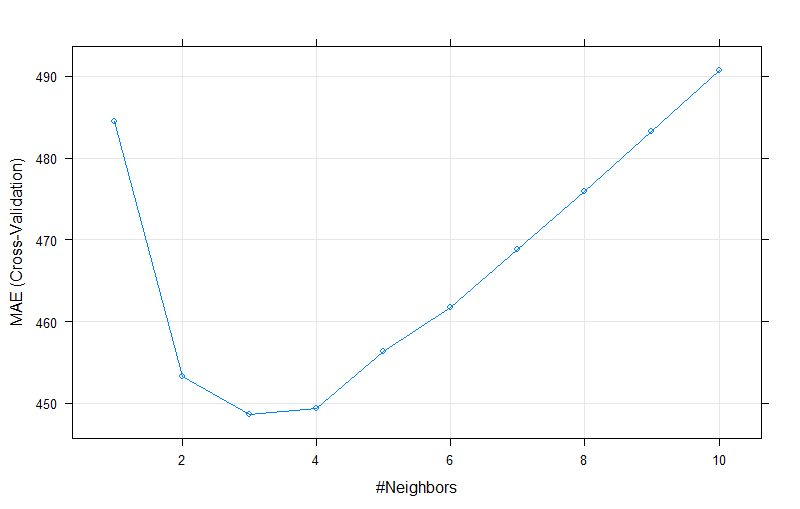
\includegraphics[scale=0.7]{imagenes/knn2.png}
	\caption{Selección del parámetro $k$ del k-NN en datos de entrenamiento y validación de DIAMONDS.}
	\label{fig:modelo2}
\end{figure}

El MAE en el conjunto de datos de prueba usando el k-NN clásico es de $432.81$ y usando el procedimiento propuesto con una cantidad de clústeres de $K = \dfrac{n-ln}{2}$ y $l = 0.75$ se obtiene un MAE de $531.35$. En este caso los resultados no son tan satisfactorios como en el MNIST. Esto puede estar dado por varias razones una de ellas puede ser que el k-NN no se comparta bien para este dataset y la otra es que no se realizó un trabajo previo de los datos antes de aplicar ambos algoritmos. A pesar de esta diferencia podemos ver en la figura \ref{fig:final2} cómo se compartan ambos métodos para una selección de observaciones de los datos de prueba ilustrando que las predicciones de ambos procedimientos son coherentes. 

\begin{figure}[H]
	\centering
	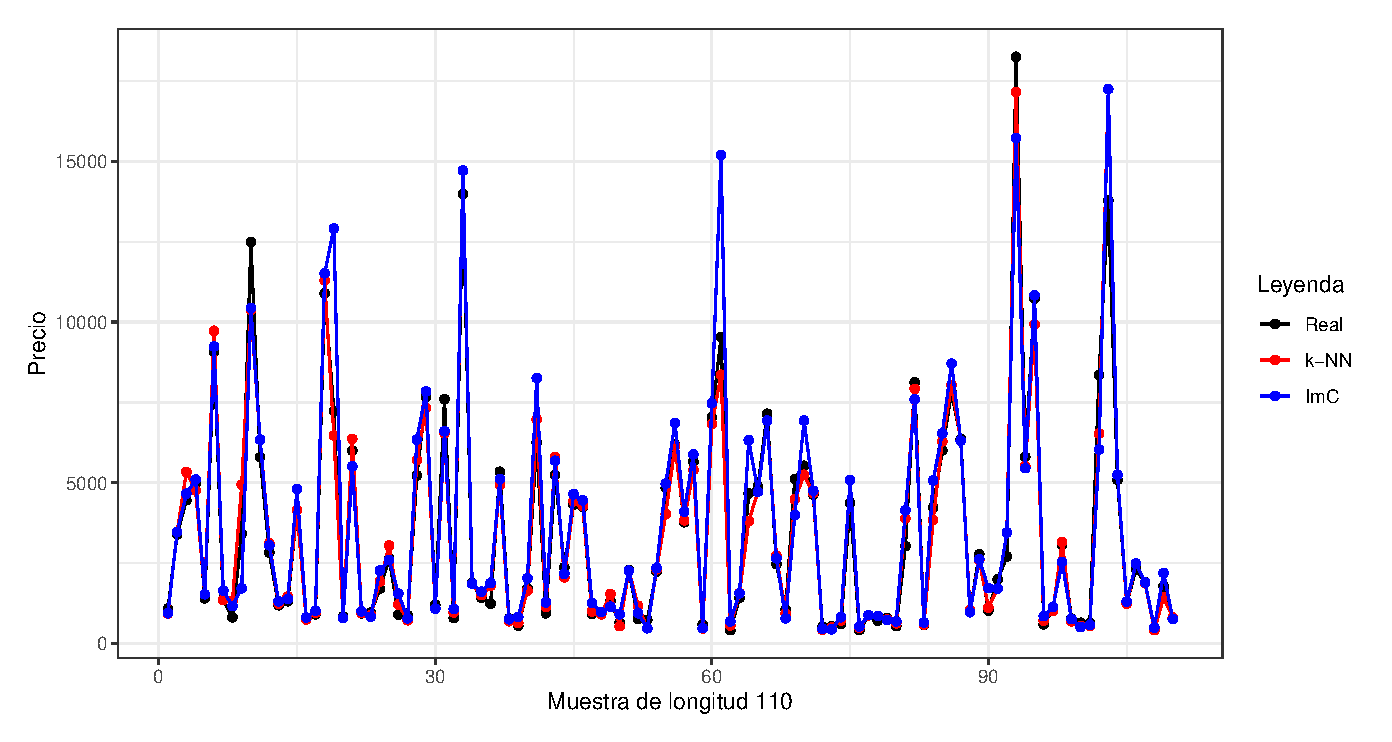
\includegraphics[scale=0.6]{imagenes/finaldiamonds.eps}
	\caption{Comparación de una muestra entre k-NN, imputación mediante clústeres y valores reales de DIAMONDS}
	\label{fig:final2}
\end{figure}


\chapter{Conclusiones y extensiones}

\section{Conclusiones}

En este trabajo fin de máster hemos estudiado modificaciones al procedimiento k-NN cuando no es factible calcular todas las distancias entre las nuevas observaciones y todas las observaciones en el conjunto de entrenamiento.\\

Hemos estudiado la combinación del algoritmo triangle fixing con varias propuestas de valores iniciales resultando que la propuesta basada en acotaciones obtiene mejores resultados y es computacionalmente factible en grandes conjuntos de datos.\\

Hemos comprobado que la selección de observaciones al azar en el conjunto de entrenamiento es inferior a una selección basada en clústeres tanto en índice de Jaccard como en el MAE.\\

El procedimiento de imputación basado en clústeres también resulta superior a los algoritmos aditivos y ultramétricos que han sido propuesto en relación con la inferencia filogenética.\\

Finalmente, hemos ilustrado la utilización del procedimiento propuesto en dos conjuntos de datos reales que muestran que en problemas de clasificación los resultados son similares al k-NN que utiliza todas las distancias y, en el caso, de regresión los resultados apuntan a que debemos refinar la selección de $K$ para tener en cuenta la función objetivo de la regresión.

\section{Líneas futuras de trabajo}

\begin{itemize}
\item Implementar estos algoritmos en un lenguaje más rápido como \textbf{\textsf{C}} o \textbf{\textsf{C++}} haciendo uso del paquete \textit{Rcpp}\cite{Rcpp} lo que permitiría realizar experimentos en conjuntos de datos de mayor dimensión.

\item Buscar un número ``óptimo'' de clústeres que tenga en cuenta la función de pérdida del problema a resolver con k-NN, es decir, que maximice la precisión en el caso del problema de clasificación o que minimice el error de predicción en el problema de regresión. También puede ser interesante estudiar la selección conjunta del parámetro $k$ del k-NN y del parámetro $K$ del procedimiento de imputación mediante clústeres.

\end{itemize}

%----------
%	BIBLIOGRAFÍA
%----------	
\newpage
\bibliographystyle{IEEEtran}
\bibliography{reference}

\chapter{Apéndice: Calendario del trabajo fin de máster}
En la siguiente tabla se mostrará el tiempo invertido en la realización de este trabajo fin de máster.

\begin{table}[H]
	\centering
	\caption{Calendario}
	\begin{tabular}{|c|c|c|c|}
		\hline
Objetivo                               & Duración & Comienzo   & Fin        \\ \hline
Estudio de la literatura               & 32 días  & 1-02-2019  & 5-03-2019 \\ \hline
Análisis preliminares de métodos       & 40 días  & 6-03-2019  & 15-04-2019 \\ \hline
Desarrollo y depuración de los códigos & 26 días  & 16-04-2019 & 12-05-2019 \\ \hline
Simulación                             & 59 días  & 13-05-2019 & 11-07-2019  \\ \hline
Análisis de datos reales               & 19 días  & 12-07-2019 & 31-07-2019 \\ \hline
Escritura y revisión de la tésis       & 30 días  & 1-08-2019  & 31-08-2019 \\ \hline
	\end{tabular}
\end{table}

\end{document}
